% This is a template for Ph.D. dissertations in the UCI format.
% 
% All fonts, including those for sub- and superscripts, must be 10
% points or larger.  Recommended sizes are 14-point for chapter
% headings, 12-point for the main body of text and figure/table
% titles, and 10-point for footnotes, sub- and super-scripts, and text
% in figures and tables.
%
% Notes: Add short title to figures, sections, via square brackets,
% e.g. \section[short]{long}.
%
\documentclass[12pt,fleqn]{ucithesis}

% A few common packages
\usepackage{amsmath}
\usepackage{amsthm}
\usepackage{array}
\usepackage{graphicx}
\usepackage[numbers]{natbib}
\usepackage{relsize}
\usepackage{rotating}
\usepackage{pdflscape}

% Some other useful packages
\usepackage{caption}
\usepackage{subcaption}  % \begin{subfigure}...\end{subfigure} within figure
\usepackage{multirow}
\usepackage{tabularx}
\usepackage{tabulary}
\usepackage[newcommands]{ragged2e}

\usepackage{csquotes}
\usepackage{pgfplots}
\usepackage{pgfplotstable}

\usetikzlibrary{trees}

% plainpages=false fixes the "duplicate ignored" error with page counters
% Set pdfborder to 0 0 0 to disable colored borders around PDF hyperlinks
\usepackage[plainpages=false,pdfborder={0 0 0}]{hyperref}

% Uncomment the following two lines to use the algorithm package,
% which provides an algorithm environment similar to figure and table
% ("\begin{algorithm}...\end{algorithm}"). A list of algorithms will
% automatically be added in the preliminary pages. Note that you
% probably want a package for the actual code to go with this (e.g.,
% algorithmic).
%\usepackage{algorithm}
%\renewcommand{\listalgorithmname}{\protect\centering\protect\Large LIST OF ALGORITHMS}

% Uncomment the following line to enable Unicode support. This will allow you
% to enter non-ASCII characters (such as accented characters) directly without
% having to use LaTeX's awkward escape syntax (e.g., \'{e})
% NOTE: You may have to install the ucs.sty package for this to work. See:
% http://www.unruh.de/DniQ/latex/unicode/
%\usepackage[utf8x]{inputenc}

% Uncomment the following to avoid "widowing", where page breaks cause
% single lines of paragraphs to float onto the next page (this is not
% a UCI requirement but more of an aesthetic choice).
%\widowpenalty=10000
%\clubpenalty=10000

% Modify or extend these at will.
\newtheorem{theorem}{\textsc{Theorem}}[chapter]
\newtheorem{definition}{\textsc{Definition}}[chapter]
\newtheorem{example}{\textsc{Example}}[chapter]

% Macros for title, author, abstract, etc.
\thesistitle{Expertise Location Approaches and Systems in Software Engineering}

%"Dissertation" for PhD, "Thesis" for master's
\documenttitle{Thesis}

\degreename{Master of Science}

% Use the wording given in the official list of degrees awarded by UCI:
% http://www.rgs.uci.edu/grad/academic/degrees_offered.htm
\degreefield{Software Engineering}

% Your name as it appears on official UCI records.
\authorname{Zhendong Wang}

% Use the full name of each committee member.
\committeechair{David Redmiles}
\othercommitteemembers
{
  James Jones\\
  Yi Wang
}

\degreeyear{2018}

\copyrightdeclaration
{
  {\copyright} {\Degreeyear} \Authorname
}

% If you have previously published parts of your manuscript, you must list the
% copyright holders; see Section 3.2 of the UCI Thesis and Dissertation Manual.
% Otherwise, this section may be omitted.
% \prepublishedcopyrightdeclaration
% {
% 	Chapter 4 {\copyright} 2003 Springer-Verlag \\
% 	Portion of Chapter 5 {\copyright} 1999 John Wiley \& Sons, Inc. \\
% 	All other materials {\copyright} {\Degreeyear} \Authorname
% }

% The dedication page is optional
% (comment out to exclude).
% \dedications
% {
%   (Optional dedication page)
  
%   To ...
% }

\acknowledgments
{
  I would like to thank...
  
  (You must acknowledge grants and other funding assistance. 
  
  You may also acknowledge the contributions of professors and
  friends.
  
  You also need to acknowledge any publishers of your previous
  work who have given you permission to incorporate that work
  into your dissertation. See Section 3.2 of the UCI Thesis and
  Dissertation Manual.)
}


% Some custom commands for your list of publications and software.
\newcommand{\mypubentry}[3]{
  \begin{tabular*}{1\textwidth}{@{\extracolsep{\fill}}p{4.5in}r}
    \textbf{#1} & \textbf{#2} \\ 
    \multicolumn{2}{@{\extracolsep{\fill}}p{.95\textwidth}}{#3}\vspace{6pt} \\
  \end{tabular*}
}
\newcommand{\mysoftentry}[3]{
  \begin{tabular*}{1\textwidth}{@{\extracolsep{\fill}}lr}
    \textbf{#1} & \url{#2} \\
    \multicolumn{2}{@{\extracolsep{\fill}}p{.95\textwidth}}
    {\emph{#3}}\vspace{-6pt} \\
  \end{tabular*}
}

% Include, at minimum, a listing of your degrees and educational
% achievements with dates and the school where the degrees were
% earned. This should include the degree currently being
% attained. Other than that it's mostly up to you what to include here
% and how to format it, below is just an example.
%
% CV is required for PhD theses, but not Master's
% comment out to exclude
% \curriculumvitae
% {

% \textbf{EDUCATION}
  
%   \begin{tabular*}{1\textwidth}{@{\extracolsep{\fill}}lr}
%     \textbf{Doctor of Philosophy in Computer Science} & \textbf{2012} \\
%     \vspace{6pt}
%     University name & \emph{City, State} \\
%     \textbf{Bachelor of Science in Computational Sciences} & \textbf{2007} \\
%     \vspace{6pt}
%     Another university name & \emph{City, State} \\
%   \end{tabular*}

% \vspace{12pt}
% \textbf{RESEARCH EXPERIENCE}

%   \begin{tabular*}{1\textwidth}{@{\extracolsep{\fill}}lr}
%     \textbf{Graduate Research Assistant} & \textbf{2007--2012} \\
%     \vspace{6pt}
%     University of California, Irvine & \emph{Irvine, California} \\
%   \end{tabular*}

% \vspace{12pt}
% \textbf{TEACHING EXPERIENCE}

%   \begin{tabular*}{1\textwidth}{@{\extracolsep{\fill}}lr}
%     \textbf{Teaching Assistant} & \textbf{2009--2010} \\
%     \vspace{6pt}
%     University name & \emph{City, State} \\
%   \end{tabular*}

% \pagebreak

% \textbf{REFEREED JOURNAL PUBLICATIONS}

%   \mypubentry{Ground-breaking article}{2012}{Journal name}

% \vspace{12pt}
% \textbf{REFEREED CONFERENCE PUBLICATIONS}

%   \mypubentry{Awesome paper}{Jun 2011}{Conference name}
%   \mypubentry{Another awesome paper}{Aug 2012}{Conference name}

% \vspace{12pt}
% \textbf{SOFTWARE}

%   \mysoftentry{Magical tool}{http://your.url.here/}
%   {C++ algorithm that solves TSP in polynomial time.}

% }

% The abstract should not be over 350 words, although that's
% supposedly somewhat of a soft constraint.
\thesisabstract
{
Successful software engineering activities require qualified software developers with proper expertise. Although expertise has been studied for many years and various expertise location approaches have been postulated, new approaches and opportunities are emerging today because of the rise of code hosting and knowledge sharing sites. As a step towards understanding the past work and the present opportunities in the context of today's software engineering practice, we perform a systematic literature survey. In analyzing the literature, we identify two broad categories of expertise research: 1) identifying the characteristics of experts, and 2) locating experts. The studies in the latter category can be further classified into three subcategories, which are: i) locating expertise by leveraging the organizational setting; ii) by mining historical artifacts; and iii) by knowledge sharing. Our analysis also identifies the major limitations of existing work, including a disconnect between early expertise studies and current location approaches; an over reliance on the experience-based model to measure expertise; a neglect on the constraints for coordination; and a lack of empirical evaluation in the real-world context, among others. Finally, we highlight research trends and promising directions for future research.
}


%%% Local Variables: ***
%%% mode: latex ***
%%% TeX-master: "thesis.tex" ***
%%% End: ***


% Add PDF document info fields
\hypersetup{
	pdftitle={\Thesistitle},
	pdfauthor={\Authorname},
	pdfsubject={\Degreefield},
}

% Uncomment the following to have numbered subsubsections (by default
% numbering goes only to subsections).
%\setcounter{secnumdepth}{4}


% Set this to only select a subset of the includes directives below.
% Very handy to speed up compilation if you're working on a certain
% part of your thesis. It conserves page numbers, references, etc.
% even for non-included files.
%\includeonly{chapter1}
\title{Expertise Location Methods in Software Engineering, a Survey}

\begin{document}

% Preliminary pages are always loaded (TOC, CV, etc.)
\preliminarypages

% Include the different components of your thesis, in separate files.
% Using \include allows you to set \includeonly above.
\chapter{Introduction}

Thriving with automation, the fields of artificial intelligence and machine learning are fundamentally changing software and conventional industries. The advance of these fields is transforming the way that we work and live. Human labor in automated routine tasks is replaced by machines and algorithms, but in other cases, automation is amplifying human labor, including in Software Engineering.

An easily neglected factor is that Software Engineering is a human centered activity \cite{fischer2003desert}, and effectively managing human resource may greatly enhance the project productivity and collaboration quality \cite{brooks1995mythical}. Hence, successful software engineering activities require qualified developers with proper expertise in order to complete the task efficiently with higher than average performance. 

A crucial aspect of managing human resource is locating expertise. Experts are able to recall their previous experience in similar work \cite{bilalić2017neuroscience,ericsson2006cambridge} with outstanding information process ability \cite{Simon:1996:SA:237774}. Various tasks in professional software development, such as, employees training and hiring, locating best personnel to perform product maintenance, and collaboration among teammates, all may benefit from effective expertise location \citep{bergersen2014construction}. However, there is still a lack of general understanding on expertise location approaches and techniques from a systematic review perspective. To further investigate this issue, we also intend to explore how can these location techniques be evaluated effectively in software engineering practice.

To address the above practical problem, this survey study reviews related literature on expertise location approaches and systems within the field of Software Engineering and Computer Supported Collaborative Work, in order to explore the application of location techniques in Software Engineering practice. From this study, we aim to picture the brief history of the development of location techniques, particularly of automated recommender systems, and evaluate the state-of-the-art research.

We take a systematic review strategy for this literature survey study. We compile a literature repository of 120 studies by querying four major online digital libraries (ACM Digital Library, Elsevier ScienceDirect, IEEE Xplore, Springer Link). We perform our literature review analysis through a six-step process, including steps of citation searching (snowball sampling), and manual literature addition based on experts suggestions, etc. After applying our review protocol and examining studies within our literature repository, 48 are identified as primary based on their research focuses (corresponding to the research question of this study) and impact to the field.

By summarizing a view for the developing history of expertise location approaches and systems, we found that the granularity of the expertise location approaches has been becoming smaller, which are from performing a general jobs to finishing a specific task. According to the analysis on our literature repository, we identified two board categories of expertise research. The first category expertise research identifies the characteristics of expertise \cite{ericsson2006cambridge, MCKEITHEN1981307, soloway1984empirical}. These studies conducted field observation \cite{mcdonald1998just} to explore how experts communicate and solve problems in the real-world context. Further other studies employed lab experiments to empirically compare the difference between expert and novice based on their behavior while completing programming tasks \cite{MCKEITHEN1981307}. The second category aims to locate expertise through various approaches. This category can be further classified into three subcategories, locating expertise by leveraging the organizational setting manually \cite{yarosh2013need}; mining historical artifacts \cite{Anvik2006who, mockus2002expertise, schuler2008mining, servant2012whosefault, fritz2010degree}; and analyzing the social network for knowledge sharing \cite{nardi2002integrating, lin2009smallblue}. As the automated location techniques developing, and the emergence of new collaborative models such as the pull request model in open source community, more specific types of expertise have been identified for open source collaboration \cite{costa2016tipmerge, yu2016reviewer, chan2016improving}. We found recent studies have shifted their focuses mostly to mining historical artifacts. In addition, as the knowledge sharing platforms emerging particularly for software engineering, there is a lack of observational study to determine the role of these Q\&A sites in expertise location activities.

% which are: locating expertise by leveraging the organizational setting; by mining historical artifacts; and by knowledge sharing.

Our review also identifies the major limitations of existing research. First, there is a disconnect between early expertise studies and current location approaches. Observation study suggested mining historical artifacts is common practice in Software Engineering, and current automated location studies tend to focus mining historical data of expert which indicates their experience \cite{servant2012whosefault,costa2016tipmerge, yu2016reviewer}. However, early cognitive studies identify the expertise based on monitoring the performance of experts \cite{MCKEITHEN1981307, soloway1984empirical, pinto1988providing}. Thus, the over-reliance on predicting a subject's performance on her past experience with code artifacts may be a threat to locate expertise precisely. Second, current location approaches neglect the constraints for experts to coordinate such as neglecting time availability and geographical distance \cite{olson2000distance}. Finally, there is a lack of empirical evaluation in real-world context, and a few studies build the ground truth of expertise to evaluate their approaches by cross validation \cite{Anvik2006who, xu2016predicting}.

Based on our review, we provide and discuss following guidelines for future studies in expertise location. Particularly, we suggest to fill the gap between early cognitive studies and location approaches, i.e., include supporting data of experts performance rather than only considering their activity record. Supporting data includes feedback from other peers and the organization or community, since these sources have watched or collaborated with the expert when performing their tasks. In addition, while designing the expertise location systems, the designer needs to beware of the \textit{paradox of expertise} \cite{dror2011paradox}, i.e., experts may be biased by their ability and their previous experience. Depending on the nature of the task, such as training and expertise sharing, the candidate with highest expertise may not always be best choice.

The remainder of the paper is organized as follows. We first present a background on the nature of expertise in Chapter 2, which includes several studies in the cognitive and neuroscience perspectives. The protocol for conducting the survey, and the evaluation matrices that we applied for all the studies in our literature repository are presented in Chapter 3. In Chapter 4, we present the result of our survey includes the major findings we mentioned above and comparison between same type of expertise research. We provide a discussion of future expertise research direction and limitation of this work in Chapter 5. At last in Chapter 6, we conclude the our study.

% \begin{figure}
% \begin{verbatim}
% #include <iostream>
% int main(int argc, char** argv) {
%   std::cout << "Hello World." << std::endl;
%   return 0;
% }
% \end{verbatim}
%   \caption{Example source code.}
%   \label{fig:sourcecode}
% \end{figure}

% \begin{table}
%   \centering
%   \begin{tabular}{|rr|r|}
%     \hline
%     $x$ & $y$ & $z$ \\
%     \hline
%     14 & 12 & -2 \\
%     0 & 33 & -25 \\
%     -3 & 11 & 22 \\
%     4 & 4 & 6 \\
%     \hline
%   \end{tabular}
%   \caption{Example coordinates.}
%   \label{tab:coordinates}
% \end{table}


%%% Local Variables: ***
%%% mode: latex ***
%%% TeX-master: "thesis.tex" ***
%%% End: ***

\chapter{Background}

Lew Platt once commented in the 1980s: ``If only HP (Hewlett-Packard\footnote{https://www.hp.com}) knew what HP  knows, we would be three times more productive.'' His words indicate that the problem of fully utilizing all expertise within an organization is desirable but hard to achieve for organizations (especially as large as HP). For a software development organization, failing to identify and select proper expertise is a threat which lowers productivity, and further overburden central individuals (\textit{expertise escalation}), e.g., core product manager, in the organization \cite{mcdonald1998just}. As the development of information technology, software engineering is vital for human beings' daily activities, and the failure of software may further threat the quality of our lives and may lead to hazard at the society level. Locating and then utilizing an organization's own \textit{intangible human resources} is a challenging two-step (location and utilization) process for all software organizations and communities \cite{bohlander2010managing}. Extracting specific domain expertise from individual talent among these organizations is the critical first step.

\section{Nature of Expertise and Expert}

To locate expertise precisely, first, we need to have a clear understanding of the nature of expertise and who have them. According to the view of a psychologist, \citeauthor{ericsson2006cambridge} define expertise as the ``\textit{characteristics, skills and knowledge}'' in a relative approach while comparing experts to novices and less experienced people \cite{ericsson2006cambridge}. Their definition illustrates that people with related expertise would have better performance than those without it.

\begin{displayquote}
``\textit{Expert: one who is very skillful and well-informed in some special field.}'' -Webster's New World Dictionary

``\textit{Experts are people who produce clearly above average (outstanding) performance on a regular basis.}'' -Cambridge handbook of Expertise and Expert Performance
\end{displayquote}

The above two definitions of expert are from Webster's New World Dictionary \cite{guralnik1983webster}, and Cambridge handbook of Expertise and Expert Performance \cite{ericsson2006cambridge} respectively. Both of them suggest a relative approach to define expert by comparing experts performance with novices. However, as previous research suggests, there is another approach to identify experts by studying genuinely exceptional people, with the goal of understanding how they perform \cite{chi2006two}.

In addition to \citeauthor{ericsson2006cambridge}'s view, from a neuroscience perspective in \citeauthor{bilalić2017neuroscience}'s research on explaining the nature of expertise \cite{bilalić2017neuroscience}, \citeauthor{bilalić2017neuroscience} classifies the expertise into categories. There are three major types of expertise when human beings are referring to the skills and specialties that expert masters:

\begin{itemize}
\item \textit{Perceptual Expertise}: This type of expertise that predominantly rely on the information directly come from human biological senses. For instance, the radiologist example mentioned in \citeauthor{bilalić2017neuroscience} mentioned, who could enable her visual expertise while detecting the problem of the patient through an X-ray photo.
\item \textit{Cognitive Expertise}: The second type of expertise focuses on the memory engagement and mental stimulation, rather than information gathering process in the perceptual expertise, such as mathematical calculation skills. Particularly, the state-of-the-art research on software engineering expertise (for example, \cite{Anvik2006who, mcdonald2000expertise, mockus2002expertise, fritz2010degree, yu2016reviewer, costa2016tipmerge}) focuses on this type of expertise when looking for programming experts.
\item \textit{Motor Expertise}: the last type of expertise is the muscle and body control ability, such as dancing, sports, playing music and other general movements. An example expert of this type could be a professional basketball player who can hit shots from long range in a higher chance than an ordinary novice.
\end{itemize}

In addition, if we look at a definition of expertise by software engineering researcher by \citeauthor{mockus2002expertise} \cite{mockus2002expertise}: 

\begin{displayquote}
``Expertise is defined as the skill of an expert, and, if interpreted quantitatively, reflects the degree of the ability of a person to perform a certain task.''
\end{displayquote}

The concept of expertise can be interpreted as a quantitative value, but in reality, it is very complicated to measure, for example, early studies in cognitive science use eyeball tracking to determine the information processing ability which is an indicator of expertise \cite{gobet1996recall}.

Another general expectation of experts is that they could utilize their expertise and previous experience to handle any unexpected situation and outcome \cite{ericsson2006cambridge}. Since experts have already acquired enough knowledge as a structured system in their \textit{long-term memory}, they would quickly adopt the situation in their field, and they also would be able to automatically provide and recognize reasonable solutions rather than figure them out.

In this study, we would cover basic approaches to locating expertise (absolute and relative), comparing their measurement of expertise, and finally evaluate these expertise location studies. Moreover, we attempt to summarize literature that considers the above two factors, i.e., memory recalling procedure, and evaluating expertise location methods.

\section{Memory Engagement and Expertise}

As this study particularly focuses the expertise and expert location in the field of programming and software engineering, the most critical type of expertise is the \textit{cognitive expertise}, though the other two types could also be involved in the software production. The connection between memory and expertise is very tight due to our memory storage system. Many studies have been conducted on the structural model of human memory, and memory/expertise retrieval mechanism. The most related ones are the \textit{Chess Experiment} for \textit{Chunking theories} \cite{chase1973perception, de2008thought, gobet1996recall} and the \textit{Amnesia Patient Experiment} \cite{cohen1980preserved}.

\begin{figure}
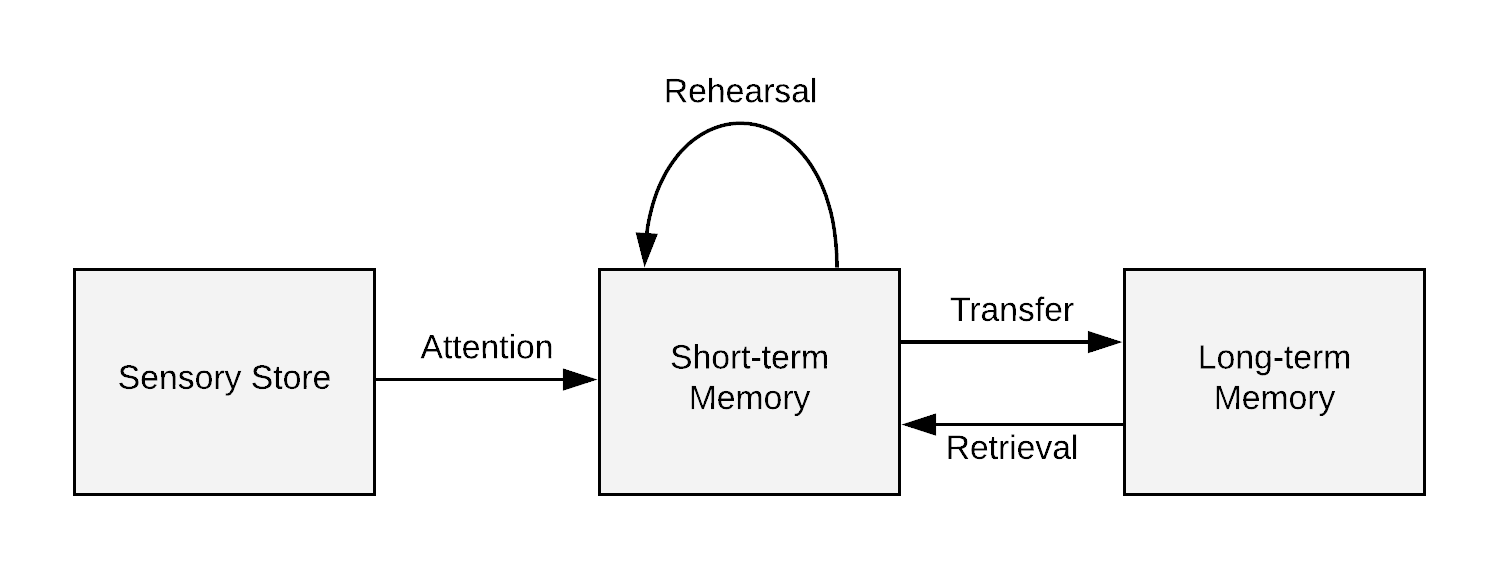
\includegraphics[width = 1\columnwidth]{memory_store.png}
\centering
\caption{The different memory sections, and the process of transferring and retrieving relation between sensory store, short-term memory and long-term memory}
\label{memoryStore}
\end{figure}

Human beings receive raw information and store it at the sensory store, but only if the information got human attention, the information would be processed to the \textit{short-term memory}, which is not everlasting and typical only stay for about 18 seconds without rehearsal \cite{revlin2012cognition}. Further, through several iterations of rehearsal, information in short-term memory would be transferred to \textit{Long-term Memory} which is the \textit{Synaptic Consolidation} process \cite{dudai2004memory}, and the information is hard to forget through a forgetting process. Therefore, the long-term memory reflection is an essential indicator of having the expertise, and cognitive literature has also supported it. 

\begin{displayquote}
Hence we can say that one part of the grand-master's chess skill resides in the 50,000 chunks stored in memory, and in the index (in the form of a structure of feature tests) that allows him to recognize any one of these chunks on the chess board and to access the information in long-term memory that is associated with it. The information associated with familiar patterns may include knowledge about what to do when the pattern is encountered. Thus the experienced chess player who recognizes the feature called an open file thinks immediately of the possibility of moving a rook to that file. The move may or may not be the best one, but it is one that should be considered whenever an open file is present. The expert recognizes not only the situation in which he finds himself but also what action might be appropriate for dealing with it.
\end{displayquote}

As mention by Simon in his masterpiece, the Science of the Artificial \cite{Simon:1996:SA:237774}, when referring to experts, we expected that they could retrieve their similar experience or expertise to solve the problem at hand, and De Groot lead studies on the expertise retrieval from long-term memory and purposed the chunking theory \cite{chase1973perception, de2008thought, gobet1996recall}. Early in 1965, De Groot conducted the chess experiment to explore the performance difference between chess experts and novices by recalling chess positions. Each participant would have 5 seconds of viewing and remember the chess board with positioned pieces and then trying to re-position all pieces on the board. However, in short, experienced expert chess players could recall more pieces and make fewer mistakes. As the progress made in neurobiology, researchers realize that information is stored in memory as chunks \cite{chase1973perception}. Chase and Simon in their following study of chess experiment, they explain the superior performance of experts with the better functioning ability of chunks. Experts could retrieve more and larger chunks from their memory of specialized field. In addition, a later study \cite{richman1995simulation} suggests that once experts encounter a new/unexpected situation in their specific domain, and then experts would automatically active their domain-specific expertise in long-term memory, which supports the second expectation for an expert in section 2.1.

\usetikzlibrary{trees}

\begin{figure}
\centering
\begin{tikzpicture}[sibling distance=10em, level distance = 5em,
  every node/.style = {shape=rectangle,
    draw, align=center}]]
  \node {Long-term Memory}
    child { node {Declarative: Fact} }
    child { node {Procedural: Skill}
        child { node {Skills} }
        child { node {Priming} }
        child { node {Conditioning} } };
\end{tikzpicture}
\caption{Knowing that (declarative) vs. Knowing how (procedural): the long-term memory model from \citeauthor{cohen1980preserved} \cite{cohen1980preserved}}
\label{LTM model}
\end{figure}

Further, it is worth noticing that, according to empirical results, there is a difference between ``knowing what'' and ``knowing how'' in human long-term memory. In 1980, Cohen and Squire conducted the study on Amnesia patients to the exam which part of patient memory or totally had been impaired \cite{cohen1980preserved}. However, the result suggested a structural model of long-term memory which is detached. The performance of patients suggests that Amnesia patients' ``knowing what'' ability is impaired, but their ability to acquire or recall (``knowing how'') skills still remain. For example, they could learn or recall how to ride a bicycle. Their study creates an initial structural model for long-term memory, and our study would refer to this series of models to analyze long-term memory reflection from surveyed literature.

\section{Expertise Location in Software Engineering}

Chunking theory can also explain the developer performance in software products based on empirical results. \citeauthor{MCKEITHEN1981307} have conducted a study on the performance difference between programming novices and experts \cite{MCKEITHEN1981307}, and it empirically confirmed that experts have superior performance throughout experiments, and also they confirmed that chunk theory still holds for programming performance, as experts can recall more programming concepts while solving the problems. In addition to information processing ability, \citeauthor{MCKEITHEN1981307} also mentioned that the organization of computer programming knowledge in experts mind are remarkably similar, but not identical. However, following up studies on expert performance fail to utilize expert similarity to locate experts.

A software system is an artifact that requires tremendous effort to develop due to its complex nature, and there is no one for all solution to increase software productivity \cite{brooks1987no}. Due to the complexity of software engineering, there are many sub-domains of expertise. Moreover, OSS libraries are increasingly used as components in other software artifacts. Hence, identification of the specific domain experts is particularly hard in the context of freely formed OSS teams.

\begin{figure}
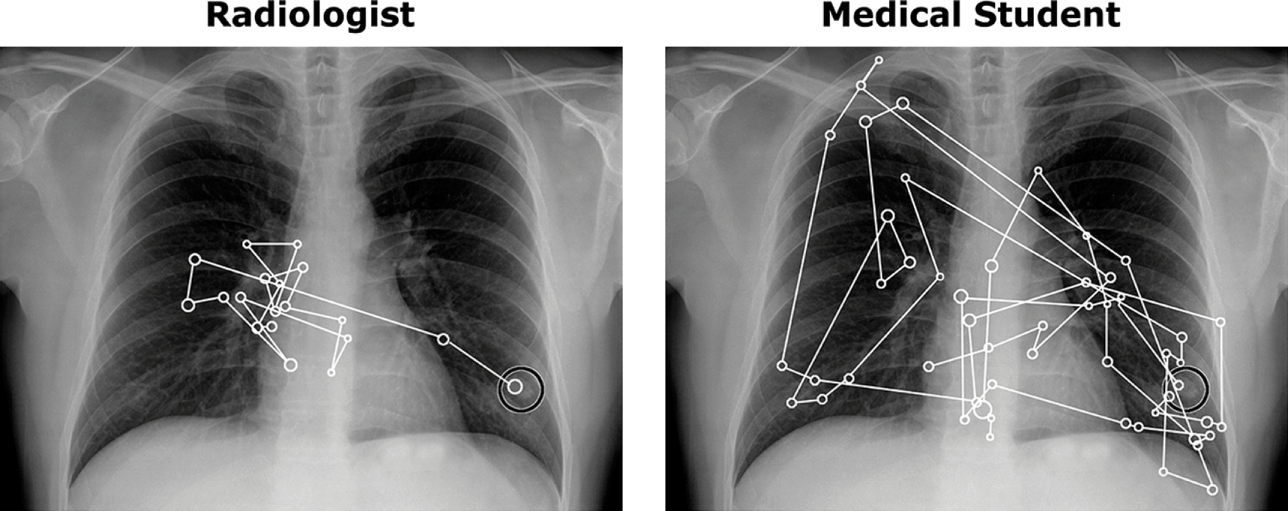
\includegraphics[width = 0.8\columnwidth]{radiologist}
\centering
\caption{The Radiologist Example That \citeauthor{bilalić2017neuroscience} Uses in \cite{bilalić2017neuroscience} Which Shows the Difference Between Experts and Novices When Processing Information}
\label{radiologist}
\end{figure}

It is a long-discussed question to define and measure expertise in a quantitative approach systematically. A quantitative approach to measure the expertise level of chess players is tracking their eyeball movement, since expert has the ability to automatically exclude irrelevant information, i.e., chess master has the capacity to focus on the most critical part of board for winning the game, but novice is not able to focus on the relevant part for planning winning strategy. Similarly, expert radiologist only needs a few glances to understand an X-ray with very few eye focus movement, but novices like medical students require more time and effort for the same process \citep{bilalić2017neuroscience}. There are several pioneer studies for locating experts in software developing process \cite{mcdonald1998just, mcdonald2000expertise, mockus2002expertise, Reichling2007}. As \citeauthor{mcdonald2000expertise} found in their studies \cite{mcdonald1998just, mcdonald2000expertise}, one of the most effective way in engineering practice identifies expert according to developer's previous experience, which could be reflected by two indicators: a developer's historical artifacts, and people whom she has worked with (her professional social network). Their work has been followed up by other researchers in software engineering, and most of their work focuses on extracting the higher precise and accurate expertise identification over historical artifacts such as code \cite{ Anvik2006who, mockus2002expertise, Servant2011history}.

Nevertheless, these expertise identification systems are considered biased due to only enabling public information, and user reputation could be easily manipulated by faking data or operating multiple accounts. However, data provided through these user-generated content enables more data sources than previous methods, and as the open source software is increasingly involved in other software engineering process, either in academia or commercial industry. The transparency provided by OSS collaboration sites could afford more activity information while locating expertise \cite{Dabbish2012social}, and distributed collaboration approach also benefit from an automated expertise identification when the team is not familiar with each other. On the other hand, precisely locating the best knowledge providers on knowledge sharing can also smooth the process with a better result.

However, in addition to mining historical artifacts, there is emerging emphasis on social networking functions for online software collaboration sites \cite{Dabbish2012social} and Q\&A knowledge sharing sites \cite{vasilescu2014social}. To encourage participant and reward contributors, these platforms provide endorsements, ratings, stars, reputation point, and other rewarding systems to acknowledge the achievement of a software developer through certification provided by her peers who use the same platform, or records in the system. 

There are a few studies \cite{hiring2016sarma} that enable these various data generated by other users. The results have suggested it is promising in hiring software developer occupations even though interviews are necessary. We will present our detailed survey results in the chapter 4.
\chapter{Approach}

After reviewing early cognitive studies on expert performance, we present this study of systematic literature review which explores the current practice of expertise location in Software Engineering. First, we illustrate the approach and protocol to conduct the review. This review is based on guidelines provided by \citeauthor{KITCHENHAM20132049} \cite{KITCHENHAM20132049}. In following sections, we specify the goals for each research question, and then provide the six-step-process in details for our review, the keywords and domains for literature searching queries: the list of literature searching engines, the standard for conference filtering, and finally the evaluation matrices for literature.

\section{Research Questions}

There are different types of experts in the field of software engineering practices. When organizers or managers intend to maximize the benefit of specific domain experts for the team goals, they need to understand the each member's expertise. To understand the capability of an organization, one of the most intuitive and efficient way is locating experts from their previous experience \cite{mcdonald2000expertise}. Due to the popularity of online open source communities, we expect to employ more data sources to generate the suggestion for locating different types of experts through rich public activity data. In this study, we survey the nature of expertise in the field of software engineering, and another goal is to review approaches from state-of-the-art expertise location research. Therefore, we purpose the following two primary research questions:\\

\fbox{\begin{minipage}{\linewidth}
\textbf{RQ1}: In the field of Software Engineering, what are the measurable characteristics that distinguish experts from novices or less-experienced subjects?
\end{minipage}}
\hfill\break
By answering the first research question, we target to conclude the characteristics that differentiate experts from less-experienced and novice developers. In addition to studies included in the background section, we also expect to learn through surveyed studies to find if there were other criteria to identify expert developer.\\

\fbox{\begin{minipage}{\linewidth}
\textbf{RQ2}: How do state-of-the-art expertise/expert location approaches and systems compile these characteristics and then locate expertise?
\end{minipage}}
\hfill\break
From the second the research question, we intend to investigate data sources and expertise models that each study adopted to determine their experts under various sub-domains. However, there are various and complex sub-domains under software engineering. When searching for various expertise location methods, we intend to examine if the model can be applied to OSS community, or if OSS public data could contribute to improving the locating quality (e.g., precision and recall) while including additional public data.

Through answering these two research questions, we expect to summarize the approaches for locating different types of expertise/experts in software engineering and provide directions to design future expertise location systems which leverage large public datasets from OSS and knowledge sharing sites. Further, use these experts as role models to guide novice software developer for their careers \cite{STEINMACHER201567}.

\section{Literature Survey Framework}

Our literature search approach is inspired by following literature survey studies in software \cite{STEINMACHER201567, Fathy2018Large}. Before starting the research process, we set up the targeted publication venues. In order to ensure the focus and quality of the literature that we are studying for constructing the initial sample, we filter out the conferences and journals other than A-ranks according to ERA\footnote{http://libguides.newcastle.edu.au/researchimpact/eralist}, Qualis\footnote{http://www.capes.gov.br/} and CCF\footnote{http://history.ccf.org.cn/sites/paiming/2015ccfmulu.pdf} these three rankings systems. In addition to the initial searching process, and we performed one round of citation searching (snowball sampling) after we constructed the initial sample. Further, at the end of sample construction, we manually added several pieces of relevant literature to our literature repository.

The overall literature selection process is as follows:

\begin{enumerate}
\item Searching digital libraries: we queried digital libraries, and then store the query result at a local paper repository which is managed by a free and open sour-source reference management tool, Zotero\footnote{https://www.zotero.org}, and it manages bibliographic data of the paper and also related copies of the paper, such as PDF files. Moreover, we use their chrome extension, Zotero Connector\footnote{https://chrome.google.com/webstore/detail/zotero-connector/ekhagklcjbdpajgpjgmbionohlpdbjgc?hl=en} to transfer the search result from web to the local paper repository.
\item Title, abstract and keywords filtering: since our query contains several generic terms in the domain of software engineering, the searching result is not promising in the recall. We perform a first level of filtering on title, abstract and keywords to check if the studies are relevant to our major objectives based on meta-data to reduce the cost of the study. From this step, we exclude most of the irrelevant papers to our research questions.
\item Introduction and conclusion analysis: then we analyze the starting and ending sections of the literature to identify their primary research goals and contribution. This part of analysis could enable us to one step further to validate whether the purpose of the subject is relevant to our research questions.
\item Citation search: for studies found relevant after all previous steps; we search on Google Scholar which aggregates literature across different resources. Then we perform the same analysis on meta-data, introduction, and conclusion to decide whether to include these studies. At this step, we dismiss the filter of Rank A conferences but include literature from all other publication venues as long as the paper is relevant to the objective.
\item Manual addition: we also include a few studies that have solid contributions to this field, especially answering our research question but not covered by the query result at the end of the study. 
\item Full literature reading: at last, if a paper is included after all previous steps, we perform a comprehensive reading throughout the paper, but also decide whether to exclude the literature in the last step.

\end{enumerate}

\begin{figure}
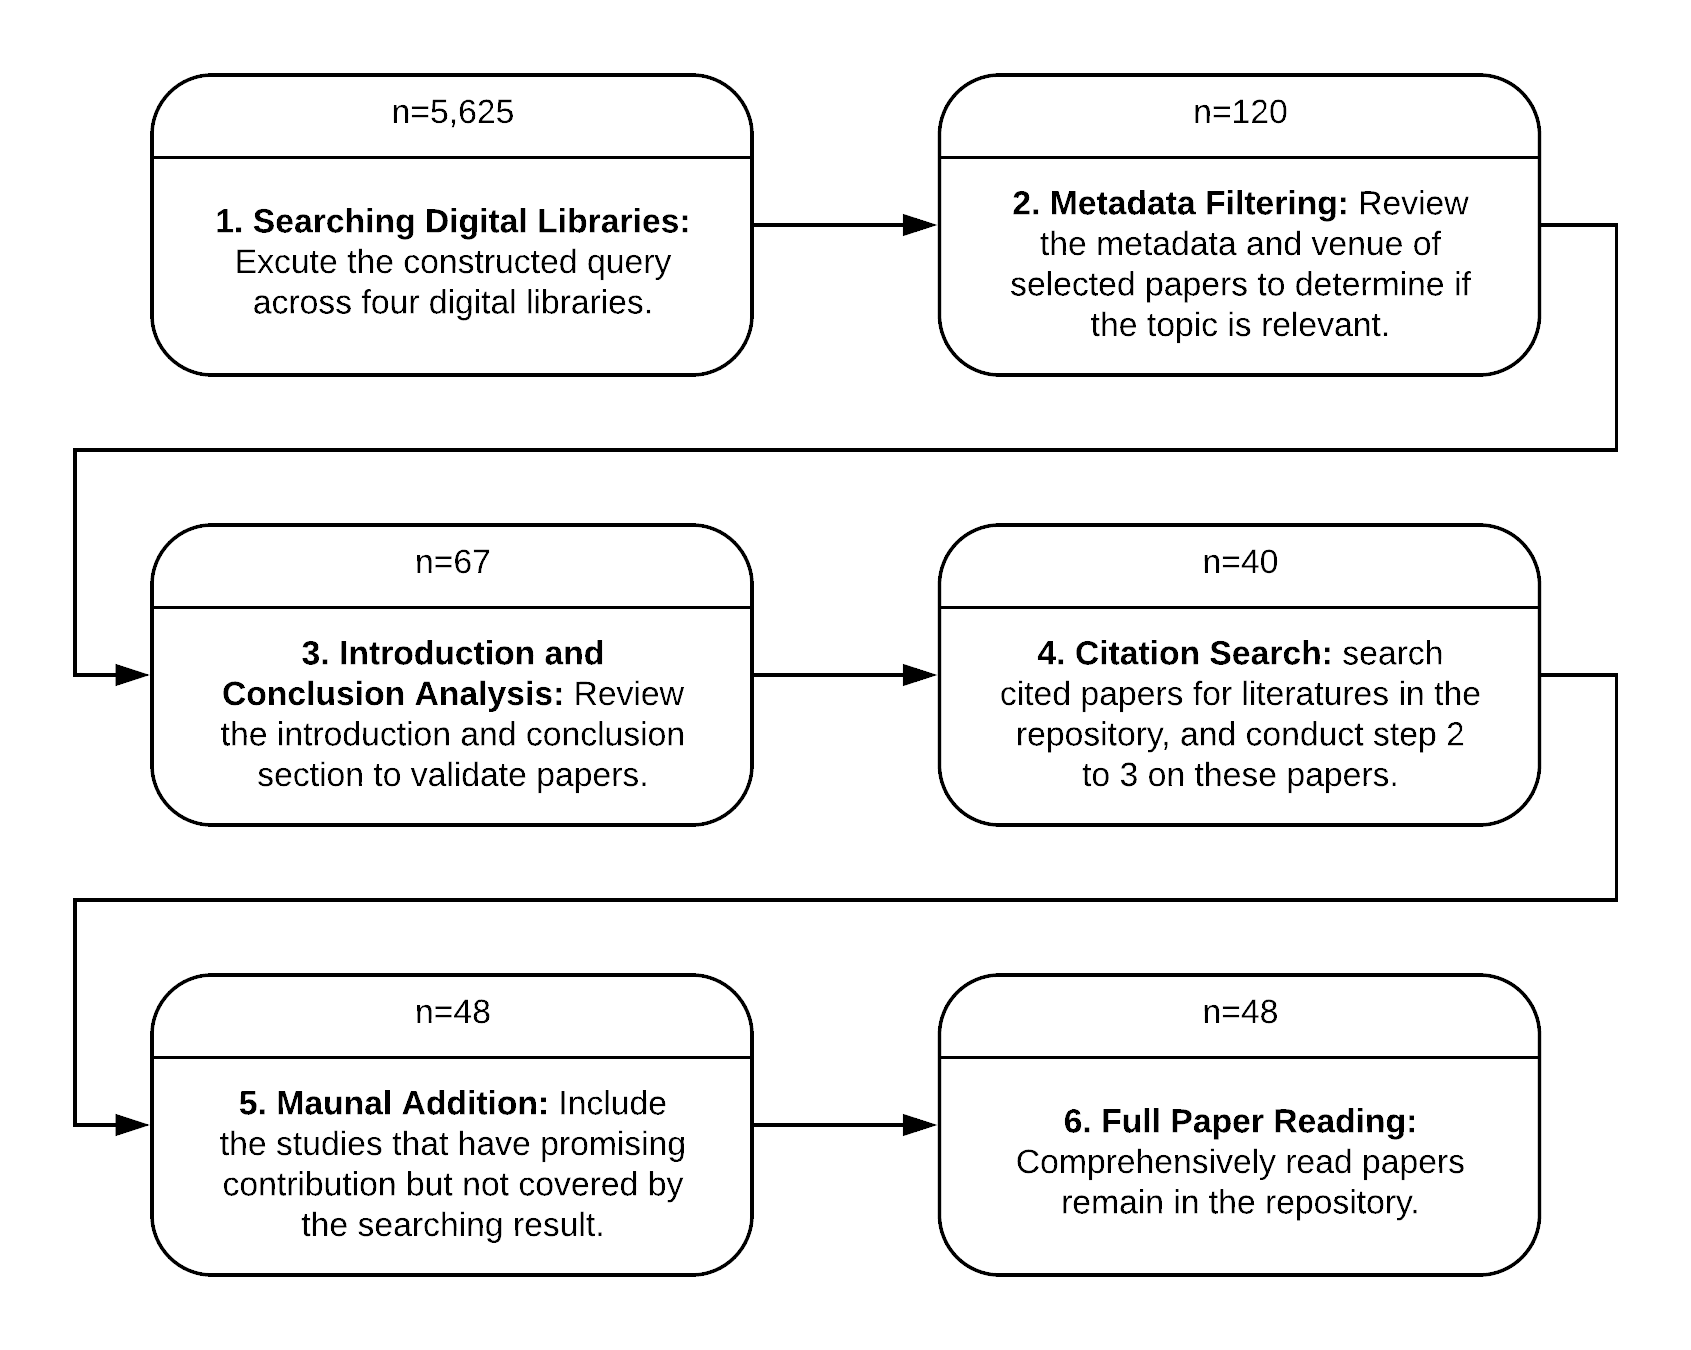
\includegraphics[width = \columnwidth]{process}
  \caption{Literature Selection Process}
  \label{fig:process}
\end{figure}

According to our research questions, we restrict our studying fields with the range of Software Engineering, Human-Computer Interaction, and Computer Supported Collaborative Work. By limiting the conferences that we are studying, we not only limited our research focuses based on RQs but also exclude papers that are not in English or not published in a peer-reviewed venue. As a result, based three publication venue ranking systems that we referred, the rank A conferences under these categories are ICSE, FSE, ASE, CSCW, and CHI; the rank A journals are IJHCS, TOCHI, TOSEM, TSE, and CSCW.

\begin{table}[tbp]
\centering
\begin{tabular}{l l}
\hline
\textbf{Item}      & {\textbf{Keyword}}                              \\ \hline
Domain I  & software, system, program          \\ 
Domain II & development, develop, engineer       \\ 
Expertise & expertise, expert, skill, knowledge \\ \hline
\end{tabular}
\caption{Keywords for Constructing the Searching Query}
\label{table:keyword}
\end{table}

We determine keywords that we would include to perform the literature search (see Table \ref{table:keyword}) upon RQ1 and RQ2. The keyword list has two major fields that we are interested in this study: domain of software engineering, and expertise location. The first set of keywords (Domain I) indicates software artifact is the subject that we concern and its synonyms. The second the set of keywords (Domain II) indicates that we are interested in expertise involved in the production procedure of software. The last set of the keywords contain the main subject of this study, expertise, and its synonyms.

The query-based textual search expression is the most available and effective mechanism to retrieve literature through digital libraries. Based on the keywords in the Table \ref{table:keyword}, we constructed a searching query connected by binary operators, which is supported by most literature search engines (see Figure \ref{fig:query}). 

\begin{figure}
\begin{verbatim}
{
  ("software" OR "system" OR "program") 
  AND 
  ("development" OR "develop" OR "engineer") 
  AND 
  ("expertise" OR "expert" OR "skill" OR "knowledge" OR "ability" OR 
  "talent")
}
\end{verbatim}
  \caption{Query Performed for Searching Literature}
  \label{fig:query}
\end{figure}

After determining the query, we select digital libraries to conduct the search. Our selection criteria are based on following: It should include major publication venue in Software Engineering, HCI, and CSCW in English, support binary operators in queries, and provide full paper access. Therefore, we selected four digital libraries to conduct our search: ACM Digital Library \footnote{https://dl.acm.org/}, IEEE Digital Library \footnote{https://ieeexplore.ieee.org/}, Scopus \footnote{https://www.scopus.com/}, and Springer \footnote{https://link.springer.com/}.

\begin{table}[tbp]
\centering
\begin{tabular}{l l}
\hline
\textbf{Conference} & \textbf{Searching Results} \\ \hline
CSCW       & 278               \\ 
ICSE       & 1451              \\ 
CHI        & 2224              \\ 
ASE        & 84                \\
FSE        & 70                \\ \hline
\end{tabular}
\caption{Searching Result of Conference Publications}
\label{table:searching_conf}
\end{table}

\begin{table}[tbp]
\centering
\begin{tabular}{ll}
\hline
\textbf{Journal} & \textbf{Searching Results} \\ \hline
CSCW    & 505               \\
IJHCS   & 811               \\ 
TOCHI   & 69                \\
TOSEM   & 92                \\
TSE     & 41                \\ \hline
\end{tabular}
\caption{Searching Result of Journal Publications}
\label{table:searching_jour}
\end{table}

\section{Literature Sampling}

\textbf{Searching Digital Libraries}: We used the query presented in Section 3.1 to retrieve an initial sample of papers, which was executed on Mar 19, 2018 across four digital libraries, and results are ordered by relevance according to each digital library.  We also used the Rank A conferences in Section 3.1 as a filter to limit result amount. See the amount initial literature sample in the table filtering by title and abstract. All queries are performed on meta-data indexing of the literature for consistency (The meta-data of a paper includes its title, abstract, and keywords).  See Table \ref{table:searching_conf} and \ref{table:searching_jour} for initial sample by publication venue from aggregated searching result. Noticeably, since we employ a reference management software to manage our paper repository and bibliographic data, it automatically to filter the duplicates of papers as we transfer the searching results into the repository in the software. Thus, there is no such a phase in our approach that removes the duplicates.

\begin{table}[tbp]
\centering
\begin{tabular}{ll}
\hline
\textbf{Conference} & \textbf{Initial Sample} \\ \hline
CSCW       & 12             \\ 
ICSE       & 39             \\ 
CHI        & 15             \\ 
ASE        & 10             \\ 
FSE        & 6              \\ \hline
\end{tabular}
\caption{Amount of Papers for Each Conference Venue in the Initial Sample}
\label{table:sample1_conf}
\end{table}

\begin{table}[tbp]
\centering
\begin{tabular}{ll}
\hline
\textbf{Journal} & \textbf{Initial Sample} \\ \hline
CSCW       & 10             \\ 
IJHCS       & 15             \\ 
TOCHI        & 1             \\ 
TOSEM        & 4             \\ 
TSE        & 8              \\ \hline
\end{tabular}
\caption{Amount of Papers for Each Journal Venue in the Initial Sample}
\label{table:sample1_jour}
\end{table}

\textbf{Meta-data Filtering}: Then based on the searching result, a researcher manually inspects the meta-data of each result to determine whether the literature is relevant to the topic. At this phase, we exclude papers that not focus on software, e.g., expertise sharing over a medical team, papers on expert systems, papers of keynote speeches and presentation notes, and also duplication. As a result, we generate an initial sample of 120 candidate papers from 5 conferences and also 5 journals. See Table \ref{table:sample1_conf} and \ref{table:sample1_jour} for numerical details by venues.

\textbf{Introduction and Conclusion Analysis}: In this step, we focus on the research methods, the contributions, and the application of studies. We exclude 53 papers which are not fitting our objectives in the research questions, for reasons such as observational study without purposing method/tool, or a study on exploring expertise in software production but without providing an approach for locating it.

\textbf{Citation Search}: After the previous step, we conduct one level of citation search (snowball sampling) on papers in the repository. We mainly focus on studies conducted by authors already in the repositories and researches with high impact (high volume of citation count provided by Google Scholar). We initially relied on the citation counts from the original digital library where the paper was found, but the result is not promising as the original library may be in lack of counting citations from publication venues are not included in this library, or even not providing a counting number. Therefore, we apply Google Scholar to search the paper again and use the citation count provided by the system to determine our initial and very brief assessment of research impacts. From this step, we include another 6 studies into our paper repository, and also we do not filter papers from publication venue standard that we used at the second step.

\textbf{Manual Addition}: There are a few important studies that are not covered by our searching query, neither could be reflected through snowball sampling. At the end of the sample construction process, we manually add a few studies that have promising research objectives or provide future directions in the field of recommending expertise. These studies are most aggregating data across multiple collaboration sites. We will provide a detailed analysis in the result section.

\textbf{Full Paper Reading}: In the last step of the sampling process, we start our analysis process while still be open to exclude studies that not focus on our research questions. As a result, we did not exclude any papers at this stage. In the following section, we will provide the evaluation matrices that we adopted during the full paper reading process. 

\section{Evaluation Matrices}

\begin{table}[tbp]
\resizebox{\columnwidth}{!}{%
\centering
\begin{tabular}{lll}
\hline
\textbf{Item}                               & \textbf{Purpose}  & \textbf{Definition}                                                                                        \\ \hline
Title                              & Overview & What is the title of the literature?                                                               \\ 
Year                               & Overview & When did the literature publish?                                                                   \\ 
Publication 
Venue                  & Overview & Where did the literature publish?                                                                  \\ 
Publication 
Type                   & Overview & What is the type of the literature (journal, conference, demo, or book)?                          \\ 
Authors                            & Overview & Who are the authors of the literature?                                                             \\ 
Research 
Type                      & Overview & What is the research approach of the literature (empirical, case study or conceptual)?            \\ 
Expertise 
Domain                   & RQ1, RQ2 & Which domain can the expertise being apply to? Software coding/testing/design etc?                \\ 
Expertise 
Model                    & RQ1, RQ2  & What is the mathematics or theoretical model of the expertise?                                      \\ 
Theory base & RQ1      & Are there any theoretical background for this model (e.g., from cognitive science/engineering/novel)? \\ 
Memory 
Engagement                  & RQ1      & Does the expertise model reflect any memory engagement associating with expertise?                \\ 
Application of Studies             & RQ2      & How does the expertise/expert location system improve the field of software engineering?          \\ 
Granularity          & RQ1, RQ2 & What is the granularity of the expertise model (element/method/file/project)?                          \\ 
Future Work             & Direction      & What is future work of this study, particularly on expertise location?                             \\ \hline
\end{tabular}
}
\caption{Evaluation Matrices for Reviewing Papers}
\label{table:evaluation}
\end{table}

While conducting the full paper reading, we set up the evaluation matrices to collect items that we are concerned according to our research question. We listed the following 13 items extracted from each literature in our paper repository (See Table \ref{table:evaluation}).

\textbf{Research overview}: There are 6 items in this category. We included the meta-data of the publication in this category like title, year, publication venue, publication type, authors and research type, especially authors of research which used for extracting primary studies in later sections. In addition to meta-data, we also identify the research types (\textit{e.g.,} conceptual, empirical, case study, ethnographic \textit{etc}.) for each paper that we reviewed. Therefore, we could summarize the suitable research methods for specific research questions in expertise studies.

\textbf{Expertise Domain}: As we mentioned in the background section 2.3, software engineering is a complex subject with multiple sub-domains. Through collecting expertise domain, we intend to investigate the status of expertise location techniques in a specific area, for example, bug report assignment, merging conflict resolution, and software fault location. We also intend to look for if there is an area that does not have an approach to locate expertise.

\textbf{Expertise Model}: We use this item to capture the conceptual or mathematical model for locating expertise. For example, Servant and Jones \cite{servant2012whosefault} use a mathematical model of \textit{speciousness} of a fault and \textit{recency} of changes on a specific line of code to determine the expertise of a developer to fix a bug. Further, an expertise model can also be represented by a very high-level conceptual model such as \cite{Ye2002Supporting} uses a four-layer model to classify the knowledge and expertise of functionality in an application. We intend to summarize approaches to locate, or even quantify expertise for software engineers in a specific domain.

\textbf{Theory Base}: We also intend to collect any theory base behind the expertise model that each study adopted. The theory can be purposed within the study based on author's suggestion, or a field study conducted before or referred from engineering or management literature. Theory bases evince the expertise model that adopted by these studies and are applicable for a larger scale.

\textbf{Memory Engagement}: Based on many studies that were referred to in the background chapter, the cognitive expertise for software engineering task is rooted in a developer's long-term memory. From this item, we intend to investigate the long-term memory reflection of expertise models, \textit{i.e.,} whether an expert determined by an expertise model was capable of reflecting information processing ability such as recalling more related memory for the subject.

\textbf{Application}: This item focuses on the application and contribution of this study. We collect this item mostly according to authors suggestion and proposal in their paper, which are usually represented in the introduction, discussion, and conclusion sections. By summarizing this item, we intend to explore our views on implications for expertise location techniques in software engineering, such as in hiring, training, and so on.

\textbf{Granularity}: The granularity of the study mainly focuses on the scale of expertise could be reflected by the model. If an expertise model utilizes the methods level coding behavior to assign developer for implementing a program method, then this model would be not applicable to determine this developer's overall knowledge on the project which contains the method. 

\textbf{Future work}: Suggestions for future directions can usually be found in discussion and conclusion sections. Although each study has its own very different purpose, from this survey, we aim to analyze and summarize the suggestions from each sub-domains and overlook a high-level future direction of expertise location approaches. 

We analyze papers in our literature repository based on the evaluation matrices listed above but not limited to. There are several cases that some of the items are not applicable to a particular study, but the overall the evaluation matrices is actionable for the majority of the studies in the paper repository.
\chapter{Results}

In this chapter, we present the results of the literature survey based on the literature repository that we constructed in Chapter 3. The literature repository is stored in the author's local computer and management by a reference management software Zotero. We extract and organize the results based on our evaluation matrices but in different categories \textcolor{red}{unclear reference of different categories} of studies. In the following subsections, we first present the overview and comparison of the literature in our paper repository, and then we summarize and highlight the most impact research in each category. Finally, we summarize findings from our review.

\section{Overview}

\textbf{Year Distribution:} Earlier research on expertise focus the cognitive science of how experts think and act. Though several directional \cite{mcdonald1998just, mcdonald2000expertise, mockus2002expertise} emerged around 2000, most follow-up studies were published in the following decade. Especially since the popularity of machine learning techniques, and to the best our knowledge, after the first study \cite{Anvik2006who} applied machine learning techniques in locating expertise for bug report assignment,  there are more studies applies statistical models via machine learning to analyze human factors in software engineering \cite{xu2016predicting, ye2014learning}. In our paper repository, most studies were published in the 2010s (See Figure \ref{yeardis}).

There are 20 journal publications and 28 conference publications respectively in venues of CSCW, Software Engineering and a few in HCI. Software Engineering has the most published papers in this repository (28 out of 48).

\pgfplotstableread[row sep=\\,col sep=&]{
    Year & Count \\
    1981 & 1 \\
    1982 & 0 \\
    1983 & 0 \\
    1984 & 1 \\
    1985 & 0 \\
    1986 & 0 \\
    1987 & 0 \\
    1988 & 1 \\
    1989 & 0 \\
    1990 & 0 \\
    1991 & 1 \\
    1992 & 0 \\
    1993 & 0 \\
    1994 & 2 \\
    1995 & 0 \\
    1996 & 0 \\
    1997 & 1 \\
    1998 & 1 \\
    1999 & 0 \\
    2000 & 1 \\
    2001 & 0 \\
    2002 & 2 \\
    2003 & 0 \\
    2004 & 0 \\
    2005 & 0 \\
    2006 & 1 \\
    2007 & 3 \\
    2008 & 2 \\
    2009 & 1 \\
    2010 & 2 \\
    2011 & 1 \\
    2012 & 5 \\
    2013 & 3 \\
    2014 & 6 \\
    2015 & 0 \\
    2016 & 9 \\
    2017 & 3 \\
    }\yeardata
\begin{figure}

    \begin{tikzpicture}
        \begin{axis}[
                ybar,
                width=\textwidth,
                height=.5\textwidth,
                nodes near coords,
                symbolic x coords={1981,1982,1983,1984,1985,1986,1987,1988,1989,1990,1991,1992,1993,1994,1995,1996,1997,1998,1999,2000,2001,2002,2003,2004,2005,2006,2007,2008,2009,2010,2011,2012,2013,2014,2015,2016,2017},
                % xtick=data,
                xtick pos=bottom,
                ytick pos=left,
                ylabel={Count},
            ]
            \addplot table[x=Year,y=Count]{\yeardata};
        \end{axis}
    \end{tikzpicture}
    \caption{Publication Year Distribution of Papers in Literature Repository}
    \label{yeardis}
\end{figure}

\textbf{Impact/Citation Count:} The average citation count of these studies is 99.4, and there are 10 studies have over one hundred citations. Hence, we argue that studies in our literature repository represent the research on expertise locations and automating this process.

\textbf{Research Type:} There are 23 empirical studies, 18 case studies, and 7 conceptual studies. Noticeably, one study conducted observation in the field to build a ground theory for expertise location method in software engineering practice \cite{mcdonald1998just}. Among these studies, 23 of them only use quantitative approaches to analyze their collected data, and 11 studies only apply qualitative approaches in their studies. Further, 7 studies apply the mixed-method to identify the evidence to support their conclusions. According to our literature repository, we found there is a variety of research methods based on their research focuses. Studies that mine historical artifacts usually apply quantitative methods to model expertise \cite{Anvik2006who, minto2007recommending, mockus2002expertise, vasilescu2014social}, and studies explore the expert characteristics and sharing expertise apply qualitative research method \cite{chen2016towards, koenemann1991expert, ley2014information, waterson1997dynamics}.

\section{Primary Studies}

In the final literature repository, we read the paper in full and then extract necessary data from each paper. Therefore, in the end, we identified these studies as primary (see Table \ref{tab:primaryStudies}) based on their focused expertise domains and correspondence to our research questions.

\begin{table}[tbp]
\centering
\begin{tabular}{llll} 
\hline
\textbf{Year}           & \textbf{Reference}          & \textbf{Year}           & \textbf{Reference} \\ \hline
\citeyear{MCKEITHEN1981307} & \citeauthor{MCKEITHEN1981307} \cite{MCKEITHEN1981307} 
& \citeyear{Dabbish2012social} &  \citeauthor{Dabbish2012social} \cite{Dabbish2012social} \\

\citeyear{soloway1984empirical} & \citeauthor{soloway1984empirical} \cite{soloway1984empirical}
& \citeyear{hanrahan2012modeling} &  \citeauthor{hanrahan2012modeling} \cite{hanrahan2012modeling} \\

\citeyear{pinto1988providing} & \citeauthor{pinto1988providing} \cite{pinto1988providing}
& \citeyear{servant2012whosefault} &  \citeauthor{servant2012whosefault} \cite{servant2012whosefault} \\

\citeyear{koenemann1991expert} & \citeauthor{koenemann1991expert} \cite{koenemann1991expert}
& \citeyear{maalej2013patterns} &  \citeauthor{maalej2013patterns} \cite{maalej2013patterns} \\

\citeyear{davies1994knowledge} & \citeauthor{davies1994knowledge} \cite{davies1994knowledge}
& \citeyear{ackerman2013sharing} &  \citeauthor{ackerman2013sharing} \cite{ackerman2013sharing} \\

\citeyear{stanislaw1994note} &  \citeauthor{stanislaw1994note} \cite{stanislaw1994note} 
& \citeyear{yarosh2013need} &  \citeauthor{yarosh2013need} \cite{yarosh2013need} \\

\citeyear{waterson1997dynamics} &  \citeauthor{waterson1997dynamics} \cite{waterson1997dynamics} 
& \citeyear{fritz2014degree} & \citeauthor{fritz2014degree} \cite{fritz2014degree} \\

\citeyear{mcdonald1998just} &  \citeauthor{mcdonald1998just} \cite{mcdonald1998just} 
& \citeyear{vasilescu2014social} &  \citeauthor{vasilescu2014social} \cite{vasilescu2014social} \\

\citeyear{mcdonald2000expertise} &  \citeauthor{mcdonald2000expertise} \cite{mcdonald2000expertise} 
& \citeyear{maalej2014comprehension} &  \citeauthor{maalej2014comprehension} \cite{maalej2014comprehension} \\

\citeyear{mockus2002expertise} &  \citeauthor{mockus2002expertise} \cite{mockus2002expertise} 
& \citeyear{ye2014learning} &  \citeauthor{ye2014learning} \cite{ye2014learning} \\

\citeyear{nardi2002integrating} &  \citeauthor{nardi2002integrating} \cite{nardi2002integrating} 
& \citeyear{ley2014information} &  \citeauthor{ley2014information} \cite{ley2014information} \\

\citeyear{chevalier2003web} &  \citeauthor{chevalier2003web} \cite{chevalier2003web} 
& \citeyear{bergersen2014construction} &  \citeauthor{bergersen2014construction} \cite{bergersen2014construction} \\

\citeyear{Anvik2006who} &  \citeauthor{Anvik2006who} \cite{Anvik2006who}
& \citeyear{chan2016improving} &  \citeauthor{chan2016improving} \cite{chan2016improving} \\

\citeyear{minto2007recommending} &  \citeauthor{minto2007recommending} \cite{minto2007recommending} 
& \citeyear{xu2016predicting} &  \citeauthor{xu2016predicting} \cite{xu2016predicting} \\

\citeyear{anvik2007determining} &  \citeauthor{anvik2007determining} \cite{anvik2007determining} 
& \citeyear{thongtanunam2016revisiting} &  \citeauthor{thongtanunam2016revisiting} \cite{thongtanunam2016revisiting} \\

\citeyear{Reichling2007} &  \citeauthor{Reichling2007} \cite{Reichling2007} 
& \citeyear{yu2016reviewer} &  \citeauthor{yu2016reviewer} \cite{yu2016reviewer} \\

\citeyear{yang2008social} &  \citeauthor{yang2008social} \cite{yang2008social} 
& \citeyear{costa2016tipmerge} &  \citeauthor{costa2016tipmerge} \cite{costa2016tipmerge} \\

\citeyear{schuler2008mining} &  \citeauthor{schuler2008mining} \cite{schuler2008mining}
& \citeyear{rahman2016correct} &  \citeauthor{rahman2016correct} \cite{rahman2016correct} \\

\citeyear{lin2009smallblue} &  \citeauthor{lin2009smallblue} \cite{lin2009smallblue} 
& \citeyear{hannebauer2016automatically} &  \citeauthor{hannebauer2016automatically} \cite{hannebauer2016automatically} \\

\citeyear{klas2010transparent} &  \citeauthor{klas2010transparent} \cite{klas2010transparent}
& \citeyear{hiring2016sarma} &  \citeauthor{hiring2016sarma} \cite{hiring2016sarma} \\

\citeyear{fritz2010degree} &  \citeauthor{fritz2010degree} \cite{fritz2010degree} 
& \citeyear{greene2016cvexplorer} &  \citeauthor{greene2016cvexplorer} \cite{greene2016cvexplorer} \\

\citeyear{gottipati2011finding} &  \citeauthor{gottipati2011finding} \cite{gottipati2011finding}
& \citeyear{lin2017improving} &  \citeauthor{lin2017improving} \cite{lin2017improving} \\

\citeyear{pipek2012bridging} &  \citeauthor{pipek2012bridging} \cite{pipek2012bridging} 
& \citeyear{saxena2017know} &  \citeauthor{saxena2017know} \cite{saxena2017know} \\

\citeyear{bednarik2012expertise} &  \citeauthor{bednarik2012expertise} \cite{bednarik2012expertise}
& \citeyear{wang2017recommending} &  \citeauthor{wang2017recommending} \cite{wang2017recommending} \\

\hline
\end{tabular}
\caption{Primary Studies in the Literature Repository}
\label{tab:primaryStudies}
\end{table}

In our literature repository, we identify two categories of expertise research: 1) identify the characteristics of experts, 2) locating experts.

% types of research
\pgfplotstableread[row sep=\\,col sep=&]{
    Type & Count \\
    Characteristics & 8 \\
    Manual & 5 \\
    Historic & 18 \\
    Sharing & 8 \\
    Network & 2 \\
    Others & 7 \\
    }\typedata
\begin{figure}

    \begin{tikzpicture}
        \begin{axis}[
                ybar,
                width=\textwidth,
                height=.5\textwidth,
                nodes near coords,
                symbolic x coords={Characteristics, Manual, Historic, Sharing, Network, Others},
                bar width = 40,
                xtick=data,
                xtick pos=bottom,
                ytick pos=left,
                ylabel={Count},
                xticklabel style = {font=\tiny},
                xticklabels={
                    Expert Characteristics,
                    Manual Location,
                    Mining Historical,
                    Sharing Content,
                    Sharing Network,
                    Others,
                },
            ]
            \addplot table[x=Type,y=Count]{\typedata};
        \end{axis}
    \end{tikzpicture}
    \caption{Publication Category Distribution of Papers in Literature Repository}
    \label{typedis}
\end{figure}

There are several early studies and a few recent studies intend to empirically identify the characteristics of experts in software engineering by monitoring their performance, see Table \ref{tab:expertCharacteristics}. There are studies explore the information processing ability of experts \cite{MCKEITHEN1981307}, the strategies that experts adopted in programming comprehension \cite{koenemann1991expert}, and validation expertise via monitoring experts performance \cite{davies1994knowledge, bergersen2014construction}.

\begin{table}[htbp]
\centering
\small
\settowidth\tymin{\textbf{Reference}}
\begin{tabulary}{\textwidth}{LLLL}
\hline
\textbf{Year}           & \textbf{Reference}          & \textbf{Approach}           & \textbf{Findings} \\ \hline
\citeyear{MCKEITHEN1981307} & \citeauthor{MCKEITHEN1981307}\cite{MCKEITHEN1981307} & Empirical Study & Experts in programming perform better in retrieving and recalling related information; experts' knowledge representations are similar.\\ \hline

\citeyear{soloway1984empirical} & \citeauthor{soloway1984empirical}\cite{soloway1984empirical} & Empirical Study & Empirically identified two types of knowledge in programming: plans and rules, which are heavily related to mind simulation and information processing. \\ \hline

\citeyear{koenemann1991expert} & \citeauthor{koenemann1991expert}\cite{koenemann1991expert} & Empirical Study & When understanding the program, experts search for relevant information in the code, and only employ a bottom-up strategy for entire program comprehension when their hypothesis failed.\\ \hline

\citeyear{davies1994knowledge} &\citeauthor{davies1994knowledge}\cite{davies1994knowledge} & Empirical Study & As the expertise growth for programming developers from lower to higher, when given a programming task, their reaction time and the number of errors made tend to be lower comparing to novices.\\ \hline

\citeyear{stanislaw1994note} &\citeauthor{stanislaw1994note}\cite{stanislaw1994note} & Empirical Study & Employ time factor, time of complete the programming task, and multitasking ability, the variety of programming skills such as the number of programming language known, to quantitatively measure expertise.\\\hline

\citeyear{maalej2014comprehension} & \citeauthor{maalej2014comprehension}\cite{maalej2014comprehension} & Case Study & Programmers comprehension strategies depends on the context, and they would avoid to understand whenever possible, similar to work of \citeauthor{koenemann1991expert}.\\\hline

\citeyear{bergersen2014construction} &\citeauthor{bergersen2014construction}\cite{bergersen2014construction} & Empirical Study & \citeauthor{bergersen2014construction} build testing model to systematically measure and valid the expertise level of programmers in Java. It validates expertise through the quality of answers and responsive time in series of programming tests, and also self-reported data of the experience and programming motivation.\\ \hline

\end{tabulary}
\caption{Primary Studies for Expert Characteristics}
\label{tab:expertCharacteristics}
\end{table}

% \begin{center}
\begin{table}[htbp]
\centering
\small
\settowidth\tymin{\textbf{Evaluation}}
\begin{tabulary}{\textwidth}{LLLLL}
\hline
\textbf{Year}           & \textbf{Reference}          & \textbf{Approach}           & \textbf{Findings}  & \textbf{Future Work}\\ \hline
\citeyear{waterson1997dynamics} & \citeauthor{waterson1997dynamics}\cite{waterson1997dynamics} & Case study: visited an IT company several times and conduct an interview-based qualitative study with key personnel in the organization & They identified the manual knowledge sharing network structure in a software development team. & Technology can be applied to the knowledge sharing process in the software development. Purpose a need of conducting case studies upon the different size of organizations to validate their structure. \\ \hline
\citeyear{mcdonald1998just} & \citeauthor{mcdonald1998just}\cite{mcdonald1998just} & Field study: conducted a field study in midsize IT company. & They found three major heuristics to locate expertise in software development practice: everyday experts, through an expertise concierge and mining historical artifacts. & Automated systems are needed to support situations in expertise location process such as the escalation behavior. \\\hline
\citeyear{pipek2012bridging} & \citeauthor{pipek2012bridging}\cite{pipek2012bridging} & Case study: longitudinal case studies in three organizations and summarize the frameworks for designing technologies for supporting expertise and knowledge management. & In expertise sharing of organizations, practice leads to technologies innovation. While integrating new tech, the new design should not disrupt the current ecosystem. & Follow the heuristics and carefully design new technologies for supporting expertise location and sharing activities. \\\hline
\citeyear{yarosh2013need} & \citeauthor{yarosh2013need}\cite{yarosh2013need} & Case study: They conducted a diary, and then interview study on professional software developers & They explore the expertise location practice, and they found in most cases (76\%) asking a colleague is the common practice to solve a problem, and tools are not helpful. & Time issue in the expertise (help) location activity. They found 15\% of the tasks involved in help-finding remained unsolved for longer than two weeks. \\\hline
\citeyear{thongtanunam2016revisiting} & \citeauthor{thongtanunam2016revisiting}\cite{thongtanunam2016revisiting} & Case Study: observe the code reviews of six software systems in the field & Majority of reviewers only contribute to one module on the system, and code reviewers with more reviewing experience are more significant in reducing the defects rather than with code authorship. & Future studies should majorly rely on using code review experience to determine best experts for reviewing the code.\\ \hline
\end{tabulary}
\caption{Primary Studies for Manual Location Approaches}
\label{tab:manual}
\end{table}
% \end{center}'

There are several studies investigated the practice of expertise location in software engineering, focusing on the common practice that manually locates experts (see Table \ref{tab:manual}). There is a study identifies the expertise sharing network structure in software development organizations \cite{waterson1997dynamics}. Moreover, there is a study identifies a set of practical strategies for locating expertise, which provides heuristics for automated expertise location systems \cite{mcdonald1998just}. Finally, there is a recent study that revisited the practices of expertise location in software organizations but found asking colleague is the most common practice, and automated location tools are hardly used \cite{yarosh2013need}.

\begin{sidewaystable}
\centering
\scriptsize
\settowidth\tymin{\textbf{Evaluation}}
\begin{tabulary}{\textwidth}{|LLLLLL|}
\hline
\textbf{Year}           & \textbf{Reference}          & \textbf{Domain}  &\textbf{Approach}  & \textbf{Evaluation}  & \textbf{Future Work}\\ \hline
\citeyear{mcdonald2000expertise} & \citeauthor{mcdonald2000expertise}\cite{mcdonald2000expertise} & Problem Casebase & Analyzing task similarity to find best expert for the current problem & Not applicable & Empirical study with developers.\\ \hline
\citeyear{mockus2002expertise} & \citeauthor{mockus2002expertise}\cite{mockus2002expertise} & Activity unit (Experience Atoms) & Accumulate the experience on historical artifacts to determine expertise & Usability test & Use time for completion to evaluate the expertise required for task; ``quantitative resume'' for developer.\\ \hline
\citeyear{Anvik2006who} & \citeauthor{Anvik2006who}\cite{Anvik2006who} & Bug report & Analyzing the Bug Report similarity and use machine learning techniques to recommend developers & Precision and recall & Empirical study with developers, additional source of information.\\ \hline
\citeyear{minto2007recommending} & \citeauthor{minto2007recommending}\cite{minto2007recommending} & Changes in historical artifacts & Apply file dependency and authorship matrix to produce expertise matrix, and finally support experts communication by locating expertise of task & Precision and recall & Empirical study with developers\\ \hline
\citeyear{anvik2007determining} & \citeauthor{anvik2007determining}\cite{anvik2007determining} & Bug Report & Empirically evaluate the expertise location approaches for bug report assignment: mining code artifacts and ``bug network''. & Precision and recall & Looking for approaches other than precision and recall to evaluate the expertise location system\\ \hline
\citeyear{Reichling2007} & \citeauthor{Reichling2007}\cite{Reichling2007} & Support Expertise Sharing & Aggregation of feedback for previous work, similarity of previous tasks and personal information. & Not applicable & Suggestion for applying technology in expertise sharing activities\\ \hline
\citeyear{schuler2008mining} & \citeauthor{schuler2008mining}\cite{schuler2008mining} & Code Artifacts & Measure expertise based on code usage data (calling) & Not applicable & Improving precision, combining with conventional authorship model, combining with task and bug reports, explore the relation between expertise and quality of work\\ \hline
\citeyear{servant2012whosefault} & \citeauthor{servant2012whosefault}\cite{servant2012whosefault} & Fault Localization & Aggregate the test cases results execution results with code modification history, and then generate the fault-to-developer assignment. & Empirically compare the WhoseFault with historical ground truth, naive methods, and other automated techniques. & Expand the WhoseFault tool with additional subjects and test cases, and also apply different mapping techniques for fault-to-developer assignment. \\\hline
\citeyear{maalej2013patterns} & \citeauthor{maalej2013patterns}\cite{maalej2013patterns} & API Documentation & List a taxonomy of knowledge type in API documentation through a four steps mix-method approach. & Case Study on two programming languages & Systematically identify the knowledge types in documentation rather than empirically. Address the gap between information seekers and providers.\\\hline
\citeyear{ye2014learning} & \citeauthor{ye2014learning}\cite{ye2014learning} & Bug Report & Employ machine learning techniques to aggregate data such as program classes name similarity and bug fixing history, and generate a list of files which are relevant to the bug. & Precision based evaluation metrics & Additional data source such as code authorship, and empirical evaluation with other projects.\\\hline
\citeyear{fritz2014degree} & \citeauthor{fritz2014degree}\cite{fritz2014degree} & Code Artifacts & Apply the Degree-of-Knowledge model to assess the expertise of a developer depending on her interaction with IDEs and code authorship (modification history) & Case Study with developers at three sites by applying the model to find experts. & Application in bug finding. Longitudinal studies with developers. Additional data source such as documentation. \\\hline
\citeyear{rahman2016correct} & \citeauthor{rahman2016correct}\cite{rahman2016correct} & Code Review & Determine code reviewer by code authorship and also experience with the collaboration model such as pull-request model on \textsc{GitHub}. &  Precision and recall, comparison with existing systems & Handling concurrent recommendation request\\\hline
\citeyear{greene2016cvexplorer} & \citeauthor{greene2016cvexplorer}\cite{greene2016cvexplorer} & Developer Profile & Retrieve developer related tags from \textsc{GitHub} activity history & Preliminary case study in two company hiring process. & Additional data source, longitudinal study in software practice, and evaluate the tool accuracy with manual extraction. \\\hline
\citeyear{costa2016tipmerge} & \citeauthor{costa2016tipmerge}\cite{costa2016tipmerge} & Merging Conflicts & Past experience of developers over different branches, and also the dependencies of modified files. & Empirical study uses historical data and compares with the actual person performed merge. & Integrate with more other algorithms, analyze in finer grain level, evaluate the project with other projects.\\\hline
\citeyear{lin2017improving} & \citeauthor{lin2017improving}\cite{lin2017improving} & Source Code Knowledge & Retrieve code-specific knowledge such API entities to support IR and learning. & Precision and recall of querying on 6 software projects & Improve document representation, additional data source and domains.\\\hline
\citeyear{wang2017recommending} & \citeauthor{wang2017recommending}\cite{wang2017recommending} & Crowdsource Assignment & Predict the skill improvement of crowd-workers based on their learning curve. & Not applicable & Finer grain of skill improvement, empirical evaluation with developers, from crowdsource to open source.\\
\hline
\end{tabulary}
\caption{Primary Studies for Mining Historical Artifacts}
\label{tab:historical}
\end{sidewaystable}

The majority of studies that automated locates expertise are designed by following the heuristic of mining historical artifacts (see Table \ref{tab:historical}). The domains of these studies are: Software problem solution, bug reports, code review, code artifacts implementation and comprehension, and so on. New techniques have been employed as they get popular in software engineering, such as machine learning, natural language processing. The most adopted method to evaluate these expertise research is precision and recall, which is a well-known method for information retrieval \cite{fawcett2006introduction}. Most studies mentioned a lack of empirical validation of their approach and purpose to aggregate more data source to improve the expertise model. There is study adopts the learning curve theory to measure the skill/expertise increases \cite{wang2017recommending}, but it still lacks evaluation to validate the approach. We are not able to identify other expertise models that measure expertise based on early theory or empirical results based on expert performance \cite{MCKEITHEN1981307, soloway1984empirical, koenemann1991expert}.

\begin{table}[htbp]
\centering
\footnotesize
\settowidth\tymin{\textbf{Evaluation}}
\begin{tabulary}{\textwidth}{LLLLL}
\hline
\textbf{Year}           & \textbf{Reference}          & \textbf{Approach}     &\textbf{Findings}  & \textbf{Future Work}\\ \hline
\citeyear{yang2008social} & \citeauthor{yang2008social}\cite{yang2008social} & Case Study with a mixmethod analysis. Particularly use Bloom Taxonomy Matrix to represent a person's expertise. & A p2p network system can support knowledge activity to effectively share knowledge, and need to locate relevant collaborators effectively. & Investigate the dynamics for different social network, and also support collaboration. \\\hline
\citeyear{gottipati2011finding} & \citeauthor{gottipati2011finding}\cite{gottipati2011finding} & Semantic search engine for finding answers, and empirical study on precision and recall, and finaly user study comparing with conventional tools. & Based on the evaluation metrics of precision and recall, and the nDCG@2 score, their approach significantly improve the answer finding experience. & Automated approach that cluster similar questions to help seekers to find relevant answers, and conduct study with other software forum.\\\hline

\citeyear{hanrahan2012modeling} & \citeauthor{hanrahan2012modeling}\cite{hanrahan2012modeling} & Case Study with Stackoverflow data & They have not yet found a strong correlation between average expertise of involved users and the duration of the time, but it is an initial attempt to model difficult of question & Conduct studies on other expert community, and use AI systems to capture critical factors of problem difficulties.\\\hline

\citeyear{vasilescu2014social} & \citeauthor{vasilescu2014social}\cite{vasilescu2014social} & Empirical study with r-Help mailing list and StackExchange data & Participants from both communities are more active than those participated one, and participants from StackExchange response faster because of the gamification. & Interview studies with participants from different communities. \\\hline

\citeyear{xu2016predicting} & \citeauthor{xu2016predicting}\cite{xu2016predicting} & Apply neural networks to find similarity between different questions in software engineering & Based on precision and recall (both lager than 0.8), their approach effectively link similar knowledge units together. & Support more data type such as code snippet and image. \\
 \hline
\end{tabulary}
\caption{Primary Studies for Knowing Sharing Sites}
\label{tab:knowledgeSharing}
\end{table}

Knowledge sharing sites are transforming the way of expertise sharing activities. Instead of locating the expert, within these platforms, finding the relevant answer which is somewhere online. Providing incentives for knowledge providers is a more focused and needed research topic, e.g., \citeauthor{vasilescu2014social} claimed the gamification features made the success of popular knowledge sharing site as StackExchange \cite{vasilescu2014social}. Further, the keyword-based search engines are not able to precisely locate the best matching question, and therefore, techniques such as semantic searching and neural networks are introduced to help the online knowledge sharing activities \cite{gottipati2011finding, xu2016predicting}.

\begin{table}[htbp]
\centering
\footnotesize
\settowidth\tymin{\textbf{Evaluation}}
\begin{tabulary}{\textwidth}{LLLLL}
\hline
\textbf{Year}           & \textbf{Reference}          & \textbf{Domain}  &\textbf{Application}  & \textbf{Visualization} \\ \hline
\citeyear{nardi2002integrating} & \citeauthor{nardi2002integrating}\cite{nardi2002integrating} & Contact Information & Support communication, and awareness of social network & Map-based visualization which clusters the people under same organization network (see Figure \ref{ContactMap}). \\\hline
\citeyear{lin2009smallblue} & \citeauthor{lin2009smallblue}\cite{lin2009smallblue} & Professional Social Network & Support awareness of social network, and visualize the expertise domain of each person. Highlight key person in the social network. & Multiple view of visualization depending on its purpose. Node tree based visualization for social network, geographic visualization for distance and availability (see Figure \ref{Smallblue}).\\
\hline
\end{tabulary}
\caption{Primary Studies for Expertise Network}
\label{tab:network}
\end{table}

A few studies are visualizing the social network of personnel in the organization. These studies support the awareness of the social network of each in it and hence support the communication among teammates. However, these studies usually do not provide evaluations of their tools, and particularly in the real-world context. Further, we are not able to find recent studies in this category.

\begin{table}[htbp]
\centering
\footnotesize
\settowidth\tymin{\textbf{Evaluation}}
\begin{tabulary}{\textwidth}{LLLLL}
\hline
\textbf{Year}           & \textbf{Reference}          & \textbf{Type}     &\textbf{Approach}  & \textbf{Findings}\\ \hline
\citeyear{pinto1988providing} & \citeauthor{pinto1988providing}\cite{pinto1988providing} & Documentation for Novice & Case Study with novices and their usage of program documentation & Novice without requisite knowledge of the program needs support of documentation, and also the presentation of the documentation matters.\\\hline
\citeyear{chevalier2003web} & \citeauthor{chevalier2003web}\cite{chevalier2003web} & Implication of Expertise Study & Empirical study with web designer at different expertise level & Web design tool should support different design strategies and remind the guideline of design for different levels of expertise respectively. \\\hline
\citeyear{klas2010transparent} & \citeauthor{klas2010transparent}\cite{klas2010transparent} & Implication of Expertise Study & Case Study with industry &  Expertise measurement can be applied to defects prediction in software product. \\\hline
\citeyear{chan2016improving} & \citeauthor{chan2016improving}\cite{chan2016improving} & Implication of Expertise Study & Empirical Study with crowd workers & Correctly facilitation experts into the crowd can help innovation and creativity in their work.\\\hline
\citeyear{hannebauer2016automatically} & \citeauthor{hannebauer2016automatically}\cite{hannebauer2016automatically} & Empirical study on location techniques & Empirical Study for comparing different automated code review assignment techniques & Automated approaches based on review experience generate better performance. \\\hline
\citeyear{hiring2016sarma} & \citeauthor{hiring2016sarma}\cite{hiring2016sarma} & Profile Aggregation & Activity Data Visualization and case study with hiring personnel & Profiles from online platforms (\textsc{GitHub} and Stackoverflow) are effective to understand a candidate's past, but interview is still needed. \\\hline
\citeyear{saxena2017know} & \citeauthor{saxena2017know}\cite{saxena2017know} & Profile Aggregation & Activity Data Visualization & Treemap visualization based on the tags provided \textsc{GitHub} and Stackoverflow. \\\hline
\end{tabulary}
\caption{Other Primary Studies}
\label{tab:other}
\end{table}

There are other studies of expertise in our literature repository, such as exploring the implications of identifying expertise level \cite{chevalier2003web, klas2010transparent, chan2016improving}, empirical studies on the performance of location techniques \cite{hannebauer2016automatically}, and expertise profile aggregation \cite{hiring2016sarma, saxena2017know}. These studies are not typical expertise location approaches but we believe they benefit this study while we build our knowledge on expertise in software.

In the following sections, we summarize several most influential studies based on their citation counts and contributions to the area of expertise location. We also report these studies in a perspective of the historical view for the development of expertise location systems and approaches.

\subsection{Expert Characteristics in Software}

\textbf{McKeithen et al. 1981}

In earlier studies, researchers confirmed that experts are generally performing better than average in their mastered fields \cite{chase1973perception, de2008thought, gobet1996recall, Simon:1996:SA:237774}. From a cogitative perspective, they found the reason is that experts can retrieve more chunks from their related memory while working on their expertise domain, which gives experts a higher information processing ability in their \textcolor{red}{unfinished sentence}.

In 1981, \citeauthor{MCKEITHEN1981307} conducted two experiments in their study. First, they tested the performance between experts and novices in computer programming tasks by letting participants to view coherent or scrambled computer programs for a 3-min recall period for 5 trials, and then participants were asked to recall everything after each trial.

The result suggests that subjects with higher expertise in computer programming, they can recall more lines of the program in either standard or scrambled versions (See Figure \ref{reitmanE1}). Their conclusion from this experiment suggested that in the field of computer programming, experts are also superior in information processing, including gathering or recalling information like other fields.

\begin{figure}
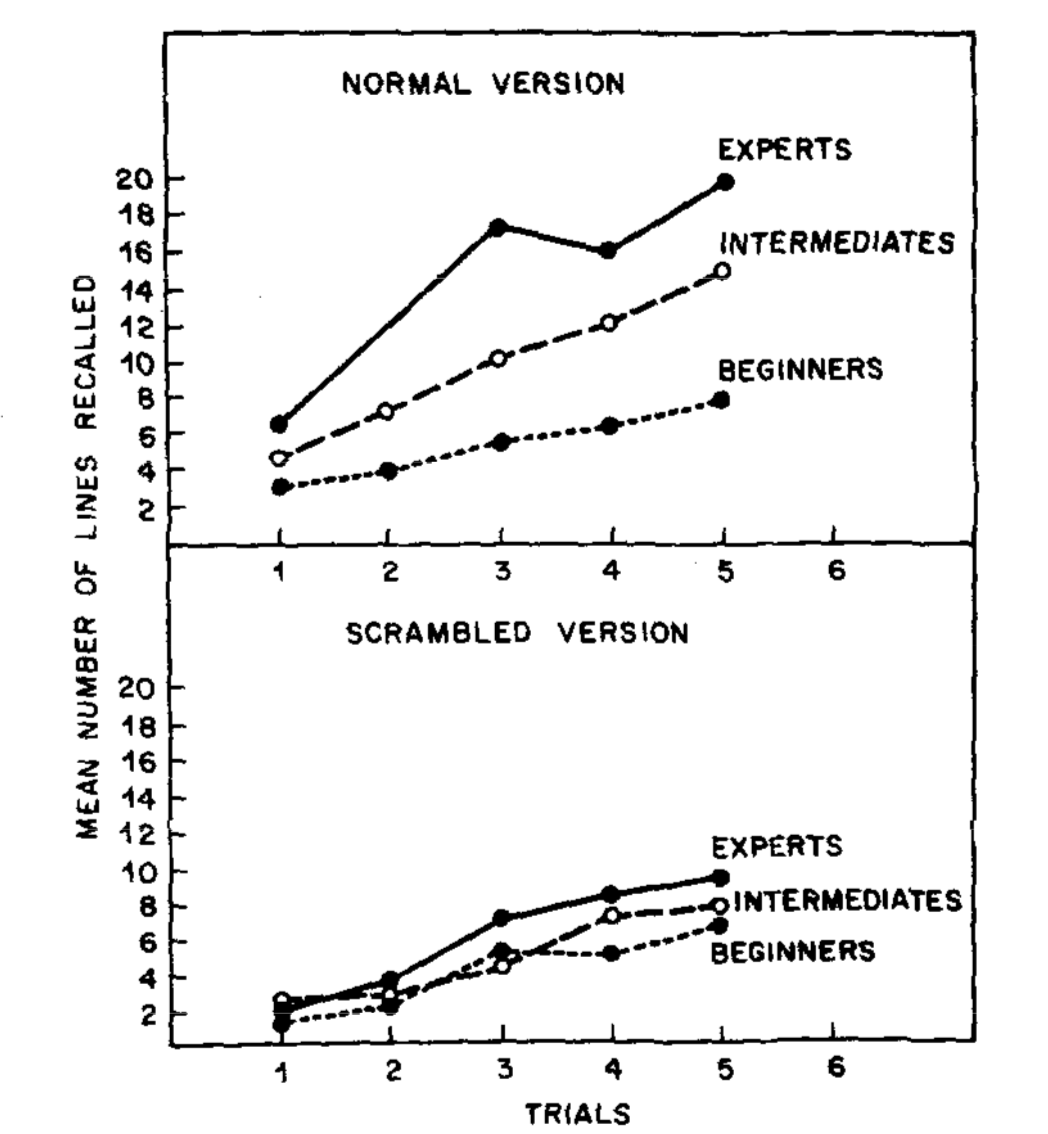
\includegraphics[width = 0.5\columnwidth]{reitmanE1.png}
\centering
\caption{Performance Differences between Experts, Intermediates and Beginners in Experiment 1 (Recalling Lines of Programs) \cite{MCKEITHEN1981307}}
\label{reitmanE1}
\end{figure}

\begin{figure}
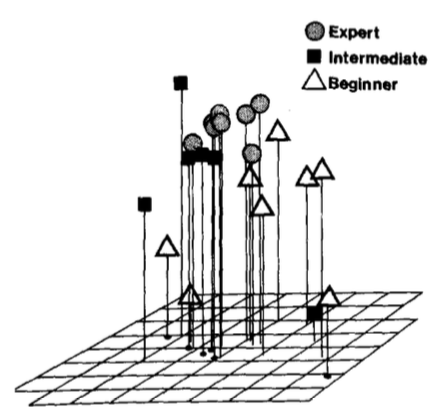
\includegraphics[width = 0.5\columnwidth]{reitmanE2.png}
\centering
\caption{Coherence between Groups of Experts, Intermediates and Beginners. Measured by Multidimensional Scaling Configuration of Distance \cite{MCKEITHEN1981307}}
\label{reitmanE2}
\end{figure}

In their second experiment, each subject was asked to organize the programming concepts in the form of hierarchical representations for keywords in computer languages such as \textsc{true, false}, \textsc{if, while} and \textsc{for}, and so on. Then they aggregated the result into a multidimensional scaling configuration for the distance between each subject. Their result suggested that experts are more cohesive to each other as a group, whose knowledge construction, i.e., the semantic representation \cite{bobrow1975representation} are particularly alike, but intermediates and beginners are not cohesive as experts (See Figure \ref{reitmanE2}).

This study has two major contributions: first, it confirmed the fact that in programming, experts are faster and precisely in processing information of computer programs which is a familiar result as in other fields. Second, it found that experts are more similar while organizing their semantic knowledge structure about programming. Moreover, in this study, expert subjects' knowledge structure have clustered a cohesive group which indicates as expertise increasing, the knowledge structure of computer programming domain will eventually be similar. 

There are a few studies later on expert characteristics and performance, such as exploring expert problem-solving strategies \cite{davies1994knowledge, koenemann1991expert}, quantifying programmer's skills \cite{stanislaw1994note}.

\subsection{Manual Expertise Location}

\textbf{McDonald and Ackerman 1998}

In early days, practitioners locate expertise to solve problems that they could not solve alone, but over manual approaches without the assistance of automated software. In 1998, McDonald and Ackerman conducted a five-month field study in a medium-sized software firm to observe practitioner's behavior in manually locating expertise within their organizational settings \cite{mcdonald1998just}.

According to their observation, three expertise \textit{identification} approaches were summarized. First, as they purposed the terminology in the paper, senior practitioners have difficulties in articulating how they know who knows a certain area, for example, a quote from their study says:

\begin{displayquote}
``You learn who's [the] most experienced in what areas. ...You just know.'' 
-Sherry
\end{displayquote}

This expertise identification approach is the \textsc{Everyday Expertise}. However, this approach is not applicable to newcomers and sometimes even to the senior member when they were unable to track everyone. The second type of expertise identification is \textsc{Historical Artifacts}. The general philosophy of this approach is finding the person who has the last authorship (change the artifact) of the artifact that related to solving the problem. However, this approach of identifying expertise is limited by the purpose or size of the change, which may falsely identify the expert.

The last approach is asking for help from an expertise concierge. In an organization, the expertise concierge is the key personnel who has very elaborated social networks and mediates many requests for information including locating expertise. Other management studies use the term of information gatekeeper \cite{allen1977managing} information mediator \cite{ehrlich1994turning} and \cite{paepcke1996information} to refer to the same role in an organization. An expertise concierge usually refers to people who were looking for information and expertise to those who may have them.

After the identification process and if there were multiple choices, the practitioners would start the process of expertise \textit{selection}. During this process, they tend to choose a person from their local social network and avoid routing to another department. Finally, the expert whom they chose to look for help might not always be the person who could offer the help due to series reasons, and this is when \textit{escalation} happens.

This study is critically important to other studies of expertise location. It purposed three main strategies to identify experts, and two of them (historical artifacts and Expertise Concierge) are directing the later studies for automated expertise identification. However, this study's research setting is a mid-size company, which did not capture the collaboration model in larger or smaller companies, especially for distributed teams. Besides, due to the age of this study and the development of knowledge sharing/transferring platforms, we argue that we need to re-evaluate our expertise location practice in the organizational settings. 

\subsection{Automated Expertise Location Techniques and Systems}

Since 2000, researchers start building systems and methods for locating the expertise based on specific needs. Notably, these studies inherit the Historical Artifacts heuristics purposed by McDonald and Ackerman \cite{mcdonald1998just}. Also, these approaches also aim to measure and quantify expertise while mining historical artifacts.

\subsubsection{Mining Historical Artifacts}

\textbf{\citeauthor{mcdonald2000expertise} 2000}

Two years later, McDonald and Ackerman published an automated expert recommendation system for solving problems in software organizations called Expertise Recommender (ER) \cite{mcdonald2000expertise}. This expertise location system attempt to decrease the workload of expertise concierge and provide alternative options. They employed their expertise locating heuristics from their previous field study, and their main strategy is based on mining the historical artifacts.

There are two basic heuristics for expertise location in ER. The first one is Change History heuristic which adopted from the ``Line 10 Rule''
from their field study \cite{mcdonald1998just}. The ER system checks for the last change of the software module in the version control system, and the developer who made the last modification would be the best candidate to ask for help.

The second heuristic is inherited from the Tech Support. It enhances the routine behavior of technical support when she faced an unfamiliar problem and starting to find a similar experience or problem in the past. Therefore, ER creates a local database for querying similar problems that happened before and associated with the person who solved them.

A user can pick the basic heuristic based on which one fits their need of the current problem, and then choose the mechanism while selecting the expert (see Figure \ref{ERUI}).

\begin{figure}
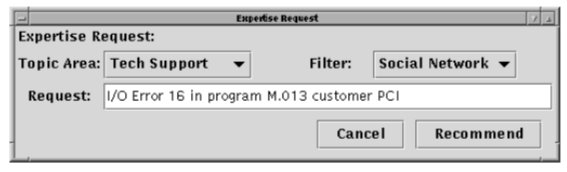
\includegraphics[width = 0.5\columnwidth]{ERUI.png}
\centering
\caption{The Expertise Request Dialog of Expertise Recommender \cite{mcdonald2000expertise}. Topic Area: Selecting the Heuristic; Filter: Strategy for Expertise Selection}
\label{ERUI}
\end{figure}

The two heuristics applied in this study are very inspiring and lead the future studies for expertise locations. Most future studies applied, integrated or combined these two heuristics for their design heuristics. For example, mine version control systems for changing history \cite{mockus2002expertise, schuler2008mining} or look for the similarity of unsolved and solved problems \cite{Anvik2006who, xu2016predicting}. This applies two data sources, changing history from the version control system and also the database of previous tech support problems. However, this system lacks a systematic evaluation or a plan on the performance of the system.

\textbf{\citeauthor{mockus2002expertise} \citeyear{mockus2002expertise}}

\citeauthor{mockus2002expertise} designed another expertise location system called \textsc{Expertise Browser} (ExB) \cite{mockus2002expertise}. Their main purpose of this study is to locate relevant expertise for collaboration in geographically distributed development. The major contribution of their work is to start quantifying a developer's expertise on specific code module based on activities and distinguish developers who have only briefly worked on a module and who have extensively worked.

In this study, they purposed a quantitative measurement of expertise without professional licensing. They defined the concept of \textit{Experience Atoms} (EAs) as the smallest unit of experience, and in practice, EAs refer to ``the smallest meaningful unit of such change,'' and the ``change'' is the direct result of a developer's activity on the product. By applying this concept, ExB summarizes a developer's expertise on changing files.

The user interface design of ExB is as follows (See Figure \ref{ExB}). For each software module, a developer would have different amounts of EAs which contribute to different levels of expertise on a specific model. In the right panel, the length of each bar on the module name represents the accumulated EAs for ``Robert Wells'' the example developer's expertise based on his activities. Intuitively, the bigger the bar represents, the higher expertise. Finally \citeauthor{mockus2002expertise} conducted a case study on distributed teams to evaluate the tool.

\begin{figure}
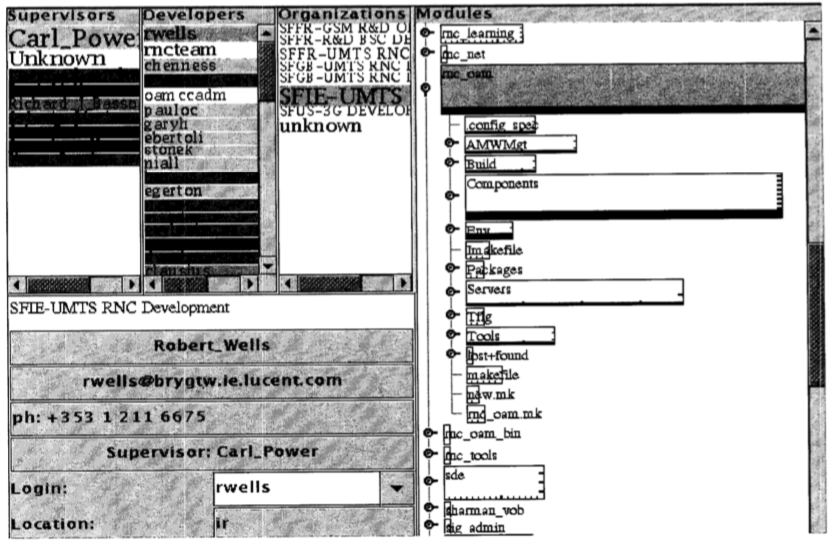
\includegraphics[width = 0.8\columnwidth]{ExB.png}
\centering
\caption{The User Interface of ExB \cite{mockus2002expertise}}
\label{ExB}
\end{figure}

Noticeably, except this study first represents the expertise in software engineering practice by the form of visualization (the area of bar charts), it gives two suggestions for future studies. First, the time of the change activity is also a critical factor to consider while building the quantitative model for expertise. In this study, the time factor is discussed to help the model the difficulty of a Modification Requests. A harder request may cause the longer time of MR interval. Though time is a critical factor in modeling and quantifying expertise, \citeauthor{mockus2002expertise} is the first to include it in the context of software engineering based on our survey \textcolor{red}{``though'' is not the right conjunction for the logic relationship you want to establish}.

In another discussion of the study, the authors were mapping experience to expertise. Though experience is not the perfect measurement for expertise, and they did not trace back to the cognitive model of expertise, their discussion provides insights on what other information can be considered in expertise measurement. Finally, they also discussed the possibility of representing a developer's expertise with visualizations. 

However, this study also has its limitation. First, it only applies the single data source, which only uses the changing log from version control system to determine the expertise. Moreover, as it is a case study, it only tested ExB's usability with participants, but it lacks user feedback or evaluation on the precision (usefulness) of the experts that ExB recommended.

\subsubsection{Expertise Concierge and Social Network Analysis}

\textbf{Nardi et al. 2002}

Earlier in 2002, information digitization has been a trend even for our contact book. As the prior work mentioned, personnel like expertise concierge plays an essential role in locating expertise under the organization setting \cite{mcdonald1998just}, but this type of role need to handle more information of other members in the team such as their contact information to find them when needs to. Thus, Nardi et al. design and implement an assistant software named ContactMap \cite{nardi2002integrating} to not only support expertise concierges to manage the contact information, and also visualize the social network of each member.

As they claimed in the paper, the major user scenarios of their tool are reminding and supporting the user. For example, reminding the user of the others' identities and connections between people in their social network, particularly the contact information of these people. In addition, ContactMap also provide \textit{awareness information} for distributed team members, such as their availability for phone calls \cite{dourish1992awareness}.

\begin{figure}
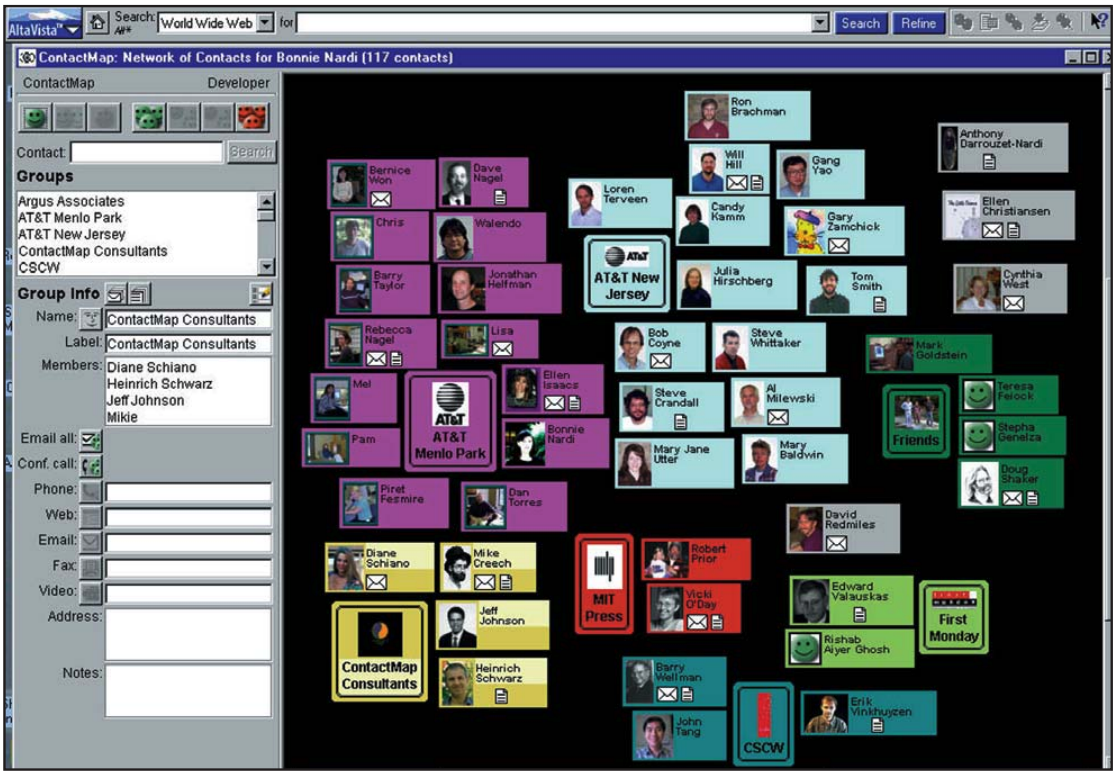
\includegraphics[width = 1\columnwidth]{ContactMap.png}
\centering
\caption{The User Interface of ContactMap \cite{nardi2002integrating}}
\label{ContactMap}
\end{figure}

This is an exploratory study of leveraging the social network of team members and support collaboration and communication. Moreover, they were also the pioneers in visualizing social networks  In the future, they plan to address more detailed research questions such as how people use this tool (evaluation of this work)?; How to support task-specific network?; Whether to hide peripheral members of the task in ContactMap and so on. They lead the discussion on this topic.

\textbf{Lin et al. 2009}

As a follow-up study on the social network analysis, Lin et al. design a social network data mining tool called Smallblue \cite{lin2009smallblue}.

In this work, they pushed the research of social network one step further by analyzing the social network and generating location of the key persons in it. They identify the key people, "Key Hubs" in the network through graph analysis such as locating structural holes. Besides the identification function, they also provide \textit{awareness information} in their tool, such as displaying the geographical information for each team member.

\begin{figure}
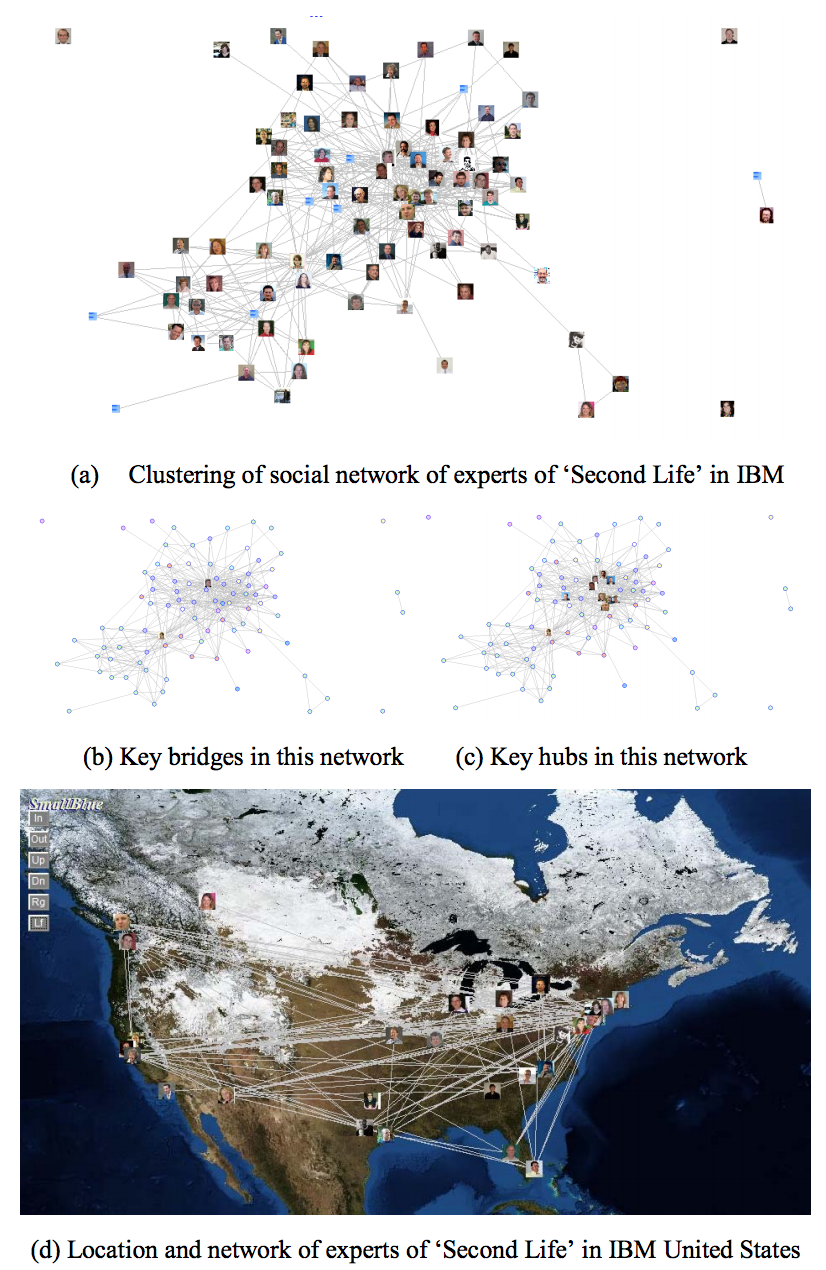
\includegraphics[width = 0.6\columnwidth]{smallblue.png}
\centering
\caption{The User Interface of Social Network in Smallblue \cite{lin2009smallblue}}
\label{Smallblue}
\end{figure}

Comparing with previous work, their visualization of a social network is more detailed in different perspectives and provide richer information on an individual team member. Moreover, it gives more personal information which is beyond contact information only. This tool combines the social network attribute and expertise. Finally, it was an online web tool\footnote{http://smallblue.research.ibm.com} which is maintained by IBM, though it is no longer maintained and offline now.

\section{Open Source and Knowledge Sharing Site}

\subsection{Empower Open Source}

In 1983, Richard Stallman launched the GNU Project with free source code sharing online. Later in 1991, Linux was released by Linus Torvalds with the license for freely modifiable source code, which significantly promoted the movement of open source software. Until 2005, the most popular decentralized version control system was created, and three years later, GitHub was launched, which fundamentally changed the development process and collaboration approach for open source projects. Later in the 2010s, studies also suggest that open source contribution is also a factor to consider in the software developer hiring process. The publicity afforded by these open source projects, dramatically promotes the development of software engineering research, particularly for empirical software engineering studies. Moreover, researchers can utilize valuable public historical data for locating expertise. 

\textbf{Anvik et al. 2006}

As the emergence of machine learning technologies in software engineering, this study by Anvik et al. started to assigning bug reports to developers based on their historical activities. The main purpose of this study is to alleviate the burden of managing bug report repository in large open source development teams.

As the first study to locate expertise by using machine learning techniques, their approach trains the machine learning algorithm based on the historical experience of a developer. Their algorithm models the types of the bug that a developer had solved before, and then based on the type of the bug report which needs to be assigned which predicts developers performance on an unsolved bug. Finally, it generates a list of developers who are considered as experts on solving such a bug. To empirically validate their tool, they analyze 3,426 bug reports for Eclipse.

To characterizing bug reports, they convert text in summary and description into feature vectors which can be trained by machine learning. They applied a set of heuristics to identify the expertise based on the bug resolving history. The basic four types of which they provided in the paper are:

\begin{itemize}
\item \textit{If a report is resolved as FIXED, it was fixed by whoever submitted the last approved patch. The person who solved it in the last approved patch has the expertise.}

\item \textit{If a report is resolved as FIXED, it was fixed by whoever marked the report as resolved. The person who marked it as resolved has the expertise.}

\item \textit{If a report is resolved as DUPLICATE, it was resolved by whoever resolved the report of which this report is a duplicate. The person who resolved the report has the expertise.}

\item \textit{If a report is resolved as WORKSFORME, it was marked by the triager \textcolor{red}{trigger?}, and it is unknown which developer would have been assigned the report. The report is thus labeled as unclassifiable at the moment.}
\end{itemize}

In their approach, they applied a systematic method to evaluate the recommendation of the bug report resolving expertise based on the principle information retrieval technique, precision, and recall. They regard expertise location process as a process of information retrieval, and the query is an unsolved bug report which would be used for search experts. However, the result is not promising at that time. They have only achieved 57\% and 64\% of precision for two projects, and recall is not over 10\% for either project. Noticeably, the ground truth for evaluation on this machine learning technique is based on cross-validation. Therefore, the developer who is identified as the expert for a bug report may not carry the expected expertise.

Though this study's result does not look so great regarding percentage numbers (especially comparing to the state-of-art bug report assignment techniques), they lead a trend of research in software engineering by applying machine learning techniques to locate expertise, and also utilize the extensive data provided in online open source repositories.

\textbf{Schuler and Zimmermann 2008}

In this study, Schuler and Zimmermann refined the model of expertise on code artifacts purposed in previous studies, especially the quantitative expertise model purposed by Audris and Hebsleb in 2002 \cite{mockus2002expertise}. In addition to quantifying the expertise based on a developer's modification on the code artifact, they also introduce the concept of \textit{usage expertise} which is more straightforward to collect.

The usage expertise is the knowledge that developers would also accumulate while using other functionality such as calling APIs, which they did not implement. They argue that while calling (using) methods, developers might not be aware of implementation details, but these developers would gain expertise on how to use a method and when a method can be used.

Including refining the model of expertise on code artifacts, this study also mentioned the application of creating an expertise profile for a developer. However, due to the limitation of mining techniques, it only provides low-level information on a developer's expertise, and still needs human interpretation to refine high-level expertise summary. Moreover, the social network of developers is hard to extract information (see Figure \ref{usage}).

\begin{figure}
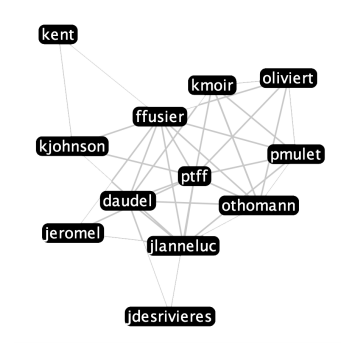
\includegraphics[width = 0.4\columnwidth]{usageExpertise.png}
\centering
\caption{An Example of Developers Usage Expertise in Their Social Network. These Developers Mostly Use the the JDT Compiler \cite{schuler2008mining}}
\label{usage}
\end{figure}

This study did not provide an evaluation or plan for your methods. However, their contribution on the quantitative model of considering what is missing at that stage is valuable, and it leads other studies to utilize the enormous data source of version control archives fully.
%rephrase it later.

\textbf{Fritz et al. 2010, 2014}

In their journal publication in 2014, Frtiz et al. summarized their work modeling expertise for code authorship and interaction. They purpose a model to capture the developer's expertise on source code element, \textit{Degree-of-knowledge}(DOK). This model utilizes the IDE to track developer's interaction with the code, and they empirically identified their results on two sites (two software development teams).

This study introduces the DOK model which represents developer's familiarity with code element. In their model, DOK is the combination of degree of authorship and degree of interest:

\begin{equation}
DOK = \alpha * DOA + \beta * DOI
\label{DOK}
\end{equation}

Particularly, the degree of authorship data is mined from version control achieves. Defined in the paper,  the degree of authorship data contains three factors (\textit{first authorship, deliveries, and acceptances}). Mylyn (was Mylar) \cite{kersten2005mylar}, an IDE plugin in Eclipse collects them as well as the degree of interaction data. The degree of interest of a code element is accumulated with each interaction the developer had with it, for example, clicking or selecting a variable name rather than editing it.

For determining the weightings, $\alpha$ and $\beta$ in the Equation \ref{DOK}, they collected the data from developers in the team, and let developer themselves to rate their knowledge about code elements as the ground truth of expertise, and then apply linear regression to decide weights in Equation \ref{DOK}.

\textbf{Servant and Jones 2012}

This paper introduces a technique called \textsc{WhoseFault} which is automated to choose expert developers to fix execution faults reflected by test cases. By applying this approach, the faulty test case can be assigned to the developer who may have the expertise to resolve the failure. Second, similar to the previous work of the second author, it provides a diagnosis of where the lines of code may cause the fault.

\begin{figure}
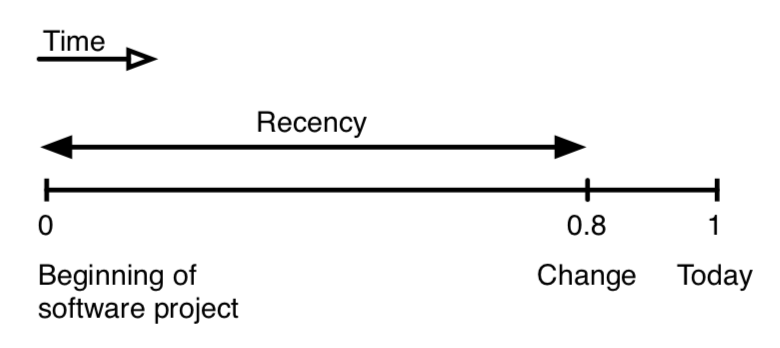
\includegraphics[width = 0.5\columnwidth]{recency.png}
\centering
\caption{The approach of calculating \textit{recency} based on the time of starting at the beginning of software project \cite{servant2012whosefault}}
\label{recency}
\end{figure}

Their approach does not only leverages the version control system to gather data but also utilizes the test cases and their execution results to complimentary the expertise model. This technique extracts the history of source code with its test cases execution result to locate the fault within the source code. It applied the same technique from their previous study \textsc{TARANTULA} to automatically local buggy code by assigning the \textit{suspiciousness} score to each line of the code \cite{jones2002visualization}. In this study, they moved one step forward to assign execution fault to developers with expertise or responsibility based on the suspicious code.

Besides \textsc{WhoseFault}'s implications on reducing bug reports generation as they claimed in the paper, this study also contributed to expertise location techniques, particularly on interpret and evaluate the quality of developer's previous working experience. Another critical contribution is that in their quantitative expertise model, they specifically consider the time factor and introduce the \textit{recency} in expertise calculation see Figure \ref{recency}. Though early study \cite{mockus2002expertise} has mentioned time would be a factor donates to the expertise measurement, but their emphasis was measurement on the difficulty of the task. 

In their evaluation, besides comparing to other similar expertise location techniques, their ground truth of expert for fixing the fault is based on the actual developer who performed the bug fixing action later. Therefore, the developer who fixed the bug is the expert. Though this method has its limitation which raises challenges such as the bug fixer may not be the best developer with the expertise, and so on. This method improves evaluation strategies, and it refers to the philosophy of evaluation approach for machine learning techniques. 

\subsection{Emergent Expert for Open Source}

\textbf{Yu et al. 2016}

The pull-request model is a widely adopted by distributed teams, especially open source ones. However, conventionally a project owner performed manually assign the developer to review the contribution, or the owner would review by herself. This manual process is time-consuming and ineffective, and it usually overburdens some team members. As a part of expertise location research, determining several best candidates for the code reviewing task is an emergent need as open source communities getting popular in software production.

In Yu's study in 2016, they purposed a method for pull-request code reviewer assignment, which automatically recommends the expert for reviewing the source code contributed in pull-request, they identification and selection procedure grounded by previous development history. Particularly, they combine their expertise factors and common interests of developers into their expertise location model.

IN addition to an experience based on the expertise model, their rationale of analyzing social interaction is based on the formation of pull-request review commit on GitHub. Since on GitHub, core team members for a software repository may not always be able or available to review the pull-request, and also because GitHub is \textit{social coding} site, outsourcing the expertise from external reviewers is usual, and they play critical roles in helping and affecting the code team members while determining whether to approve the pull-request \cite{tsay2014let}. Therefore, the interaction history of the external reviewers by comments shows their interests towards the repository, and also indirectly reflects their knowledge and expertise in the repository.

By combining this social interaction data to the experience based expertise model, they leverage the social character of the open source platforms. Noticeably, they conduct a mix method approach to evaluate their approaches. Like other recommend systems before, they adopted precision and recall to assess the performance. Moreover, they conduct a qualitative study to deeply explore the benefit of their expertise location approach by combining social interaction. Their results suggest that technical keyword in communication traces is the most relevant factor in determining the expertise of a developer to the project, and for a project has most reviews are insiders, a developer who becomes a \textit{dominant reviewer} usually leaves her communication traces in most of the pull-request. For this type of collaboration mode, one repository only has a few dominant reviewers.

\textbf{Costa et al., 2016}

Besides the pull-request model, merging is another important collaboration practice, as parallel development is beneficial to manage time to release the product either in open source communities or commercial development. However, merging is not an easy task to perform as it requires complex expertise in resolving conflicts \cite{costa2016tipmerge}. 

Current techniques and tools only detect straightforward and direct conflict such as textual conflict. However, these tools are not able to realize complex cases such as unseen dependency modifications \cite{shihab2012effect}. Therefore, it is very typical to assign a developer to manually resolve the conflict or confirm if the merge is free from potential conflicts. However, it is not clear to find the appropriate developer or locate a few experts to perform the merge action.

\begin{figure}
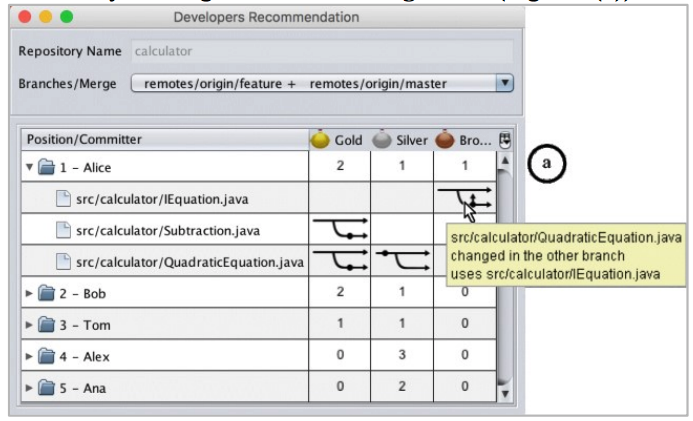
\includegraphics[width = 0.5\columnwidth]{TipMerge.png}
\centering
\caption{User Interface of Showing Rankings of Developers for Performing Merge in TipMerge \cite{costa2016tipmerge}}
\label{TipMerge}
\end{figure}

In their study, they purposed an automated approach called \textsc{TIPMerge}, a novel tool which identifies a list of developers as the best candidates to perform the merge action. Similar to other expertise location systems and approaches, it determines the expertise for performing the merge based on developer's previous experience with the branch and the project, particularly the interactions with key files for the merge and their dependencies (See Figure \ref{TipMerge}).

Finally, they evaluate their system based on a mix-method approach similar to \cite{yu2016reviewer}. They not only quantitatively compared their result with conventional methods, but also conduct a qualitative study by interviewing team members for two projects. As they summarized, there are couple reasons other than previous experience to decide a merger, such as, ``Line 10 Rule'' for merge (the developer who made the last commit would help the merge); knowledge on the trick part of the code artifact; personal preference.

\subsection{Emergence of Knowledge Sharing Sites}

Effective knowledge sharing platform has been emergent since the late 2000s (Stackoverflow launched in 2008). The free knowledge crowdsourcing practice has changed the way how developers get basic knowledge on programming questions. It was great idea and effort for Stackoverflow to organize the documents for each programming language and API, but the company has to end the project due to its enormous effort in management and low profit for return\footnote{Stackoverflow Meta, Sunsetting Documentation: https://meta.stackoverflow.com/questions/354217/sunsetting-documentation}. However, a complete documentation or code examples is necessary and affordable for private knowledge resources such as knowledge sharing repository for private companies and commercial project, for example, Software Engineer from Facebook, Satish Chandra introduced the internal code repository of Facebook on 2018 ISR research Forum at University of California, Irvine\footnote{https://isr.uci.edu/content/2018-isr-research-forum}. Properly utilize the knowledge sharing site to locate expertise is critical but the current research has been struggling with the extracting relevant information partially due to the ambiguity of natural language. Research on knowledge sharing sites is still in the beginning and building infrastructure phase.

\textbf{Hanrahan et al. 2012}

It is intuitive that a person with high expertise on the domain could answer hard related questions in software engineering, and novices in the domain could not. However, the difficulty of questions is hard to model. In this study, Hanrahan et al. employ a straightforward method to model the difficulty of a question on Stackoverflow by calculating the time duration between the problem is posted and the accepted answer is posted.

It is not a brand new idea to model the difficulty and expertise. Earlier in the study of \cite{mockus2002expertise}, they have already discussed the time issue of a task in software engineering, such as a hard request or bug would take more time to complete since it was issued. However, they did not include the time factor in their quantitative expertise model. In this study, the authors only consider the solving time as a factor, but they missed the other factors contributing to the solving time such as the popularity of the topic, question asker's representation of the question, and special cases such as adjust the question by other comments \textcolor{red}{hard to understand}. However, they provide an initial approach to model the expertise in questions through time factor.

\textbf{Xu et al. 2016}

Due to the ambiguity of natural language, and different representation may refer to the same semantic meaning, questions on Stackoverflow may be repeated or high related to each other. Removing the redundancy and simplifying the variations are critical for modeling the users' expertise and avoid information overload for knowledge providers and receivers on knowledge sharing sites. Unfortunately, Stackoverflow is not able to manage its enormous knowledge base like Wikipedia\footnote{https://www.wikipedia.org/} which links keywords, i.e., knowledge unit, to its own explanations. As the failure of Stackoverflow Documentation which is due to the nature of programming language, the complicity of programming knowledge unit is not affordable to human labor to classify.

Therefore, Xu et al. employ the convolutional neural network to model the knowledge unit in questions and answers for expertise. Through the techniques and approach described in their study, they can cluster different word representations into different high-level categories \ref{knowledgeUnit}. Besides, they also use precision and recall as the primary evaluation metrics for their approach.

\begin{figure}
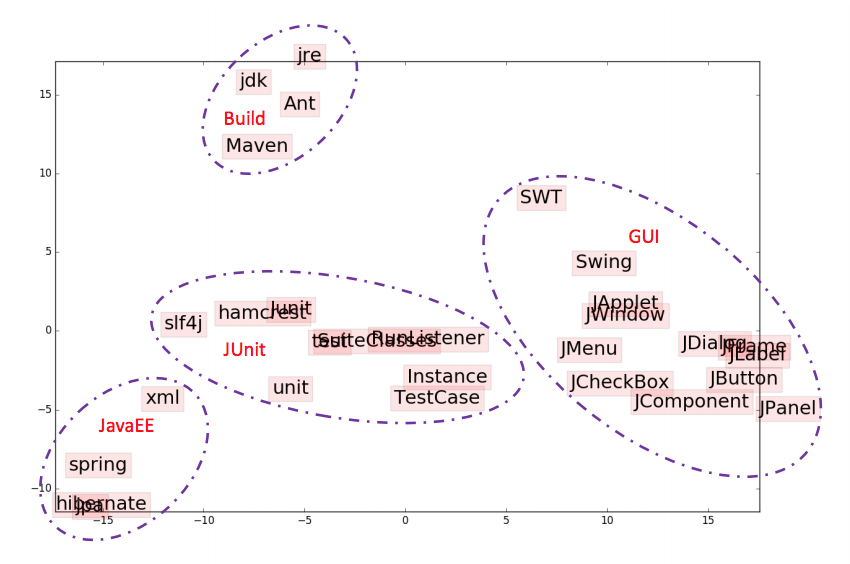
\includegraphics[width = 0.5\columnwidth]{KnowledgeUnit.png}
\centering
\caption{Word Representations Embedding Examples \cite{xu2016predicting}}
\label{knowledgeUnit}
\end{figure}

Based on their study, it is possible to manage the knowledge unit, defined in their study, and link them as Wikipedia. It enhances the usability of the site and also easier to mine a knowledge unit related expertise for developers which is at a higher level than ``tag'' in Stackoverflow.

\section{Multiplatform Data Aggregation}

\textbf{Sarma et al. 2016}

As the emerging of community-based knowledge sharing platform, e.g., Stackoveflow and open source platform, e.g., GitHub, it is necessary to monitor and aggregate a developer's activities all over the internet for precisely measuring her expertise in software engineering for both ``soft'' social skills and also technical skills.

Therefore, Sarma et al. design and implement a visualization tool, \textsc{Visual Resume} to include a developer's activities over the internet. Notably, other than the amount of the contribution for a developer over his career (bar charts in the middle of each card in Figure \ref{vr}), it also provides quality indicators of their contribution such as whether a pull-request is accepted and whether their commit passed the test cases provided in the repository. Besides, it employs a card-based user interface to allow easy comparison between developers, and mainly they design this tool to extract expertise from historical contributions for hiring purpose.

\begin{figure}
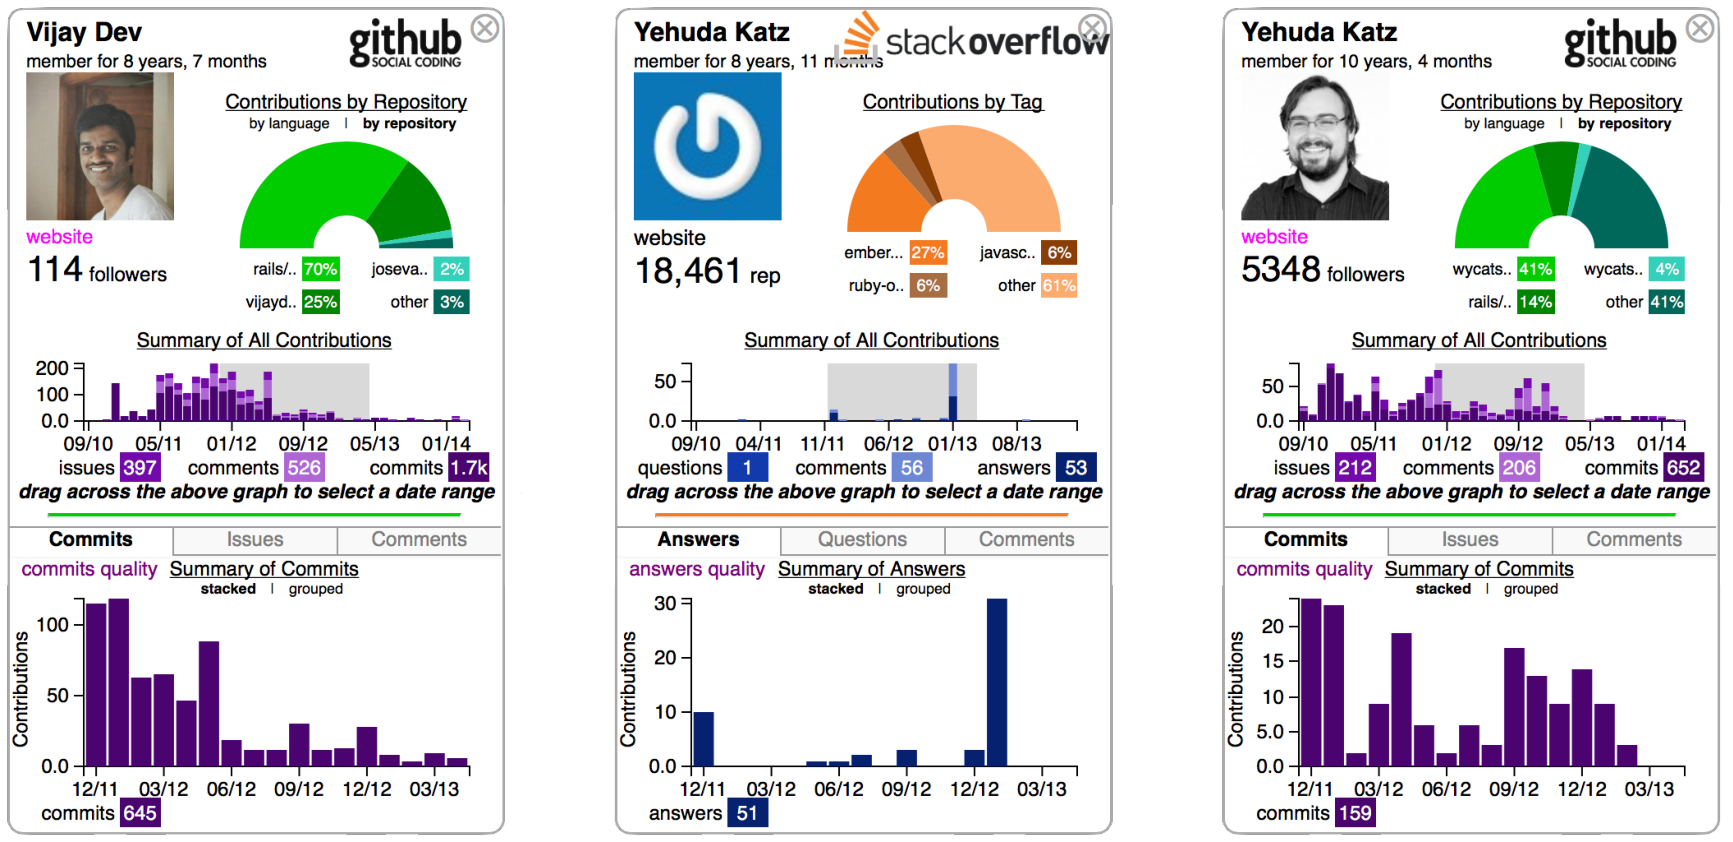
\includegraphics[width = 0.8\columnwidth]{vr.pdf}
\centering
\caption{The Card Based User Interface for Comparing Expertise in the Hiring Procedure \cite{hiring2016sarma}}
\label{vr}
\end{figure}

As for evaluation, they conduct the interview based usability test with management level of personnel from industry, and let participants either use the web portals of developer's profile or use \textsc{Visual Resume} to evaluate job candidates based on job description, and then select best candidates for the job. Particularly, other than finding \textsc{Visual Resume} is helping participants in making their decisions, participants also mentioned that the qualitative interview phase is still necessary as a part of hiring new employees.

\section{Findings Summary}

In this section, we summarize the major findings from our survey review. First, we present a historical view of expertise location systems and approaches in the development of software engineering. Further, we argue that there are some limitations to the current trend of expertise location systems, especially on their dataset to determine the expertise and evaluation methods for the system. Finally, we provide some suggestions based on the current research status.

\subsection{Evolution of Automated Techniques: From Locating Expertise of ``Playing Chess'' to ``Moving Pawn''}

In this study, we reviewed the studies of expertise location in a historical perspective. We summarize the development of expertise location studies in the figure (see Figure \ref{history}).

\begin{sidewaysfigure}[ht]
    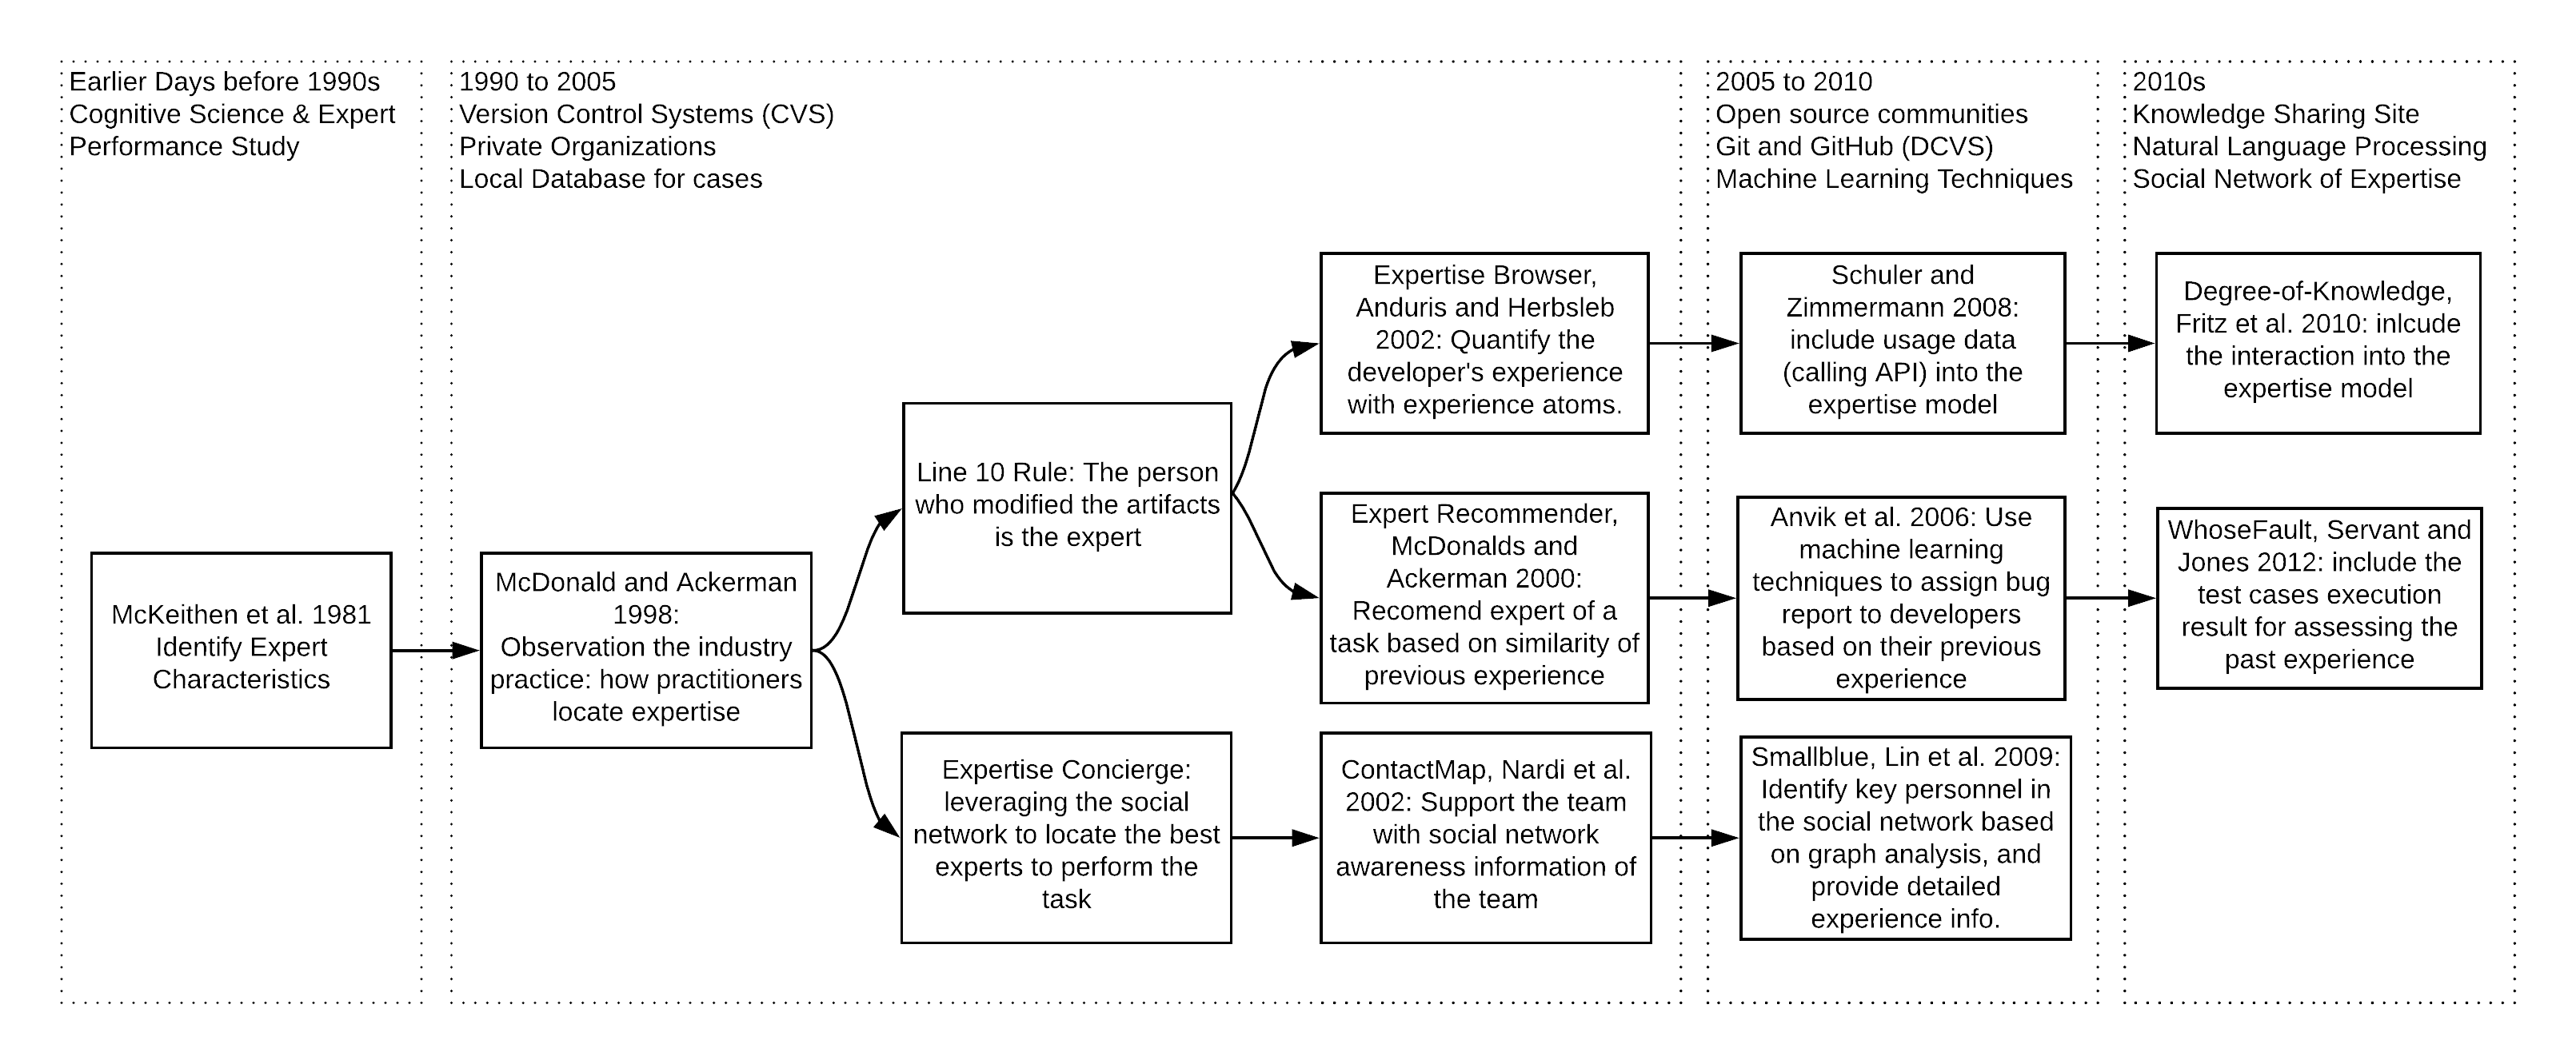
\includegraphics[width=\textwidth]{History.png}
    \caption{The Development History of Research in Expertise Location Systems and Approaches}
    \label{history}
\end{sidewaysfigure}

Early expertise research, researchers were discovering the characteristics of experts and masters, and they found experts perform better in their expertise domain mainly due to their higher information processing abilities, and this conclusion has been confirmed by a few studies in software engineering which found senior expert programmers can also process information of code faster and more precise.

Since the field study by McDonald and Ackerman in 1998 \cite{mcdonald1998just}, they set up the heuristics for expertise location systems and approaches later, mostly mining the historical artifacts or through expertise concierge. By studying our paper repository, we found automated expertise location techniques inherit and employ these two heuristics when manually locating experts. However, to the best of our knowledge, the research of expertise concierge has mostly vanished since IBM Smallblue \cite{lin2009smallblue}. On the other hand, research mines historical artifacts go to a direction of similar granularity of expertise. Automated expertise location research has a trend of going to the micro level of tasks, for example, recent research \cite{yu2016reviewer, costa2016tipmerge} focus on microtasks in open source software engineering such as merging different branches. We found the trend of going to a micro level of expertise is necessary for performing a specific low-level task (``\textit{moving pawn}''). However, when stakeholders need to perform high-level task such as locating best candidate for training and hiring new employers among candidates which require (``\textit{playing chess}''), low level expertise information closely related to programming task itself such as expertise in calling APIs is usually not intuitive to help decide the best candidates for an engineer job.

\subsection{Expertise and Time}

Only very few studies consider that expertise is not a static attribute of developers. Sarma et al. found the fact from their user study that practitioners in hiring committees of programming jobs decide a job candidate's expertise for programming task and their availability partial based on their recent activities \cite{hiring2016sarma}. Servant and Jones also consider recency as a factor in their statistical model of measuring expertise for dealing with fault, i.e., with the same amount of contribution if a developer submitted the code more recently then this developer has the higher expertise in the related issue. Early studies by \cite{mockus2002expertise} also mentioned the time issue in measuring expertise, but they intend to use the time as a measure for quantifying the difficulties and expertise required to perform the task which is under another topic. We argue that developers' expertise is continuously accumulating and diminishing. It is non-trivial to consider the time factor when measuring expertise.

\subsection{Evaluation of Expertise Location Approaches and Systems}

In this study, we found a variety of evaluation methods for expertise location approaches, but generally, previous researchers were struggling in evaluating the expertise location research and especially building the ground truth of their studies.

Earlier expertise location research usually conduct an usability test with practitioners \cite{mockus2002expertise} or even without an evaluation phase or plan \cite{nardi2002integrating, mcdonald2000expertise}. Later, \textit{Precision and Recall} becomes one of the most popular evaluation approaches to assess the effectiveness of an expertise location tool \cite{Anvik2006who, xu2016predicting, yu2016reviewer}. However, it is still hard for them to build ground truth for the result of expertise location, and cross-validation is the general solution. For example, slicing the history at a certain point of time, and uses the data before to create a reference for expertise, and then employ later data (e.g., the developer who fixed the bug) as ground truth. Though there are more factors lies between the best candidate for the task and the person who performs the task such as availability or training reasons. The complex environment and significant turnover of developers in open source projects entail more reasons of the person who performs the task in reality \textcolor{red}{unclear sentence}. However, employing the historical data is the most generic method for building the ground truth of expertise.

Due to the limitations in the evaluation of these studies, recent studies adopt a mix-method approach to build and validate the ground truth for evaluating expertise location techniques \cite{yu2016reviewer, costa2016tipmerge, xu2016predicting}. With a detailed qualitative study, these studies may be able to reveal precise expertise sharing network inside actual teams, but since the cost of these studies, researchers are not able to provide such detailed qualitative study for various environment.

\subsection{Call for a Field Study}

The last field study for locating expertise in the domain of software engineering is conducted at 1998 \cite{mcdonald1998just}, when software organizations were all private without open source communities, and also developers activities and behaviors records were stored locally inside the company. Therefore the earlier expertise location practice focus on the private data sources, including organization staff who played as key roles like expertise concierges.

However, it has been 20 years since the early field study, and both the techniques support and collaboration practice have been completely changed. The emerging techniques like machine learning techniques to support software engineering activities, natural language processing techniques to classify textual description, are significantly improving the experience of software development. New collaboration practice such as widely using the DVCS in parallel programming to save time to the market. Moreover, the internal and public knowledge sharing site is also changing the strategy of developers while transferring expertise and solving problems.

We argue that there is a need for questionnaire surveys, observations, or field studies to explore the expertise location approaches and heuristics in modern software engineering practice. Moreover, there is a need to explore the role of open source communities, knowledge sharing sites, professional social network and automated expertise location tools in the model software development. The future study shall be conducted for different purposes of expertise location studies such as hiring, training, and performing tasks.
\chapter{Discussion}

In this section, we provide several points of discussion for this study, including identifying the disconnection between discussions on the potential improvement of the expertise model, and other data sources to include to fill the gap between cognitive research and expertise location studies in software engineering. \textcolor{red}{Not sure what you want to say here, consider breaking it into simple sentences}

\section{``How Well Do They Perform'' v.s. ``What Have They Done''}

By reviewing our repository, we found that the quantitative expertise model has continuously been evolving, which adds new data sources, such as adding interaction data \cite{fritz2010degree}, and including API usage data \cite{schuler2008mining} into their expertise measurement model. However, these expertise models still have failed to measure the cognitive characteristics of experts, which were identified by early cognitive studies \cite{MCKEITHEN1981307, Simon:1996:SA:237774, gobet1996recall}. Based on these previous researches, experts process, i.e., receive and recall, their domain information faster and more precisely, which grants their higher proficiency in their domains. The excellence of their information processing ability helps them to realize the best solution and handle unexpected situation \cite{ericsson2006cambridge} automatically. The conclusion from these cognitive studies is evidenced by empirical studies which monitoring the experts' performance while doing the task (monitoring how well expert perform). However, the heavy experience-based expertise models (measuring what experts have done) fail to reflect developers ability in processing information in the field of software engineering. We argue that there is a \textbf{disconnect} between early cognitive studies on expert performance and the software engineering approaches and systems for locating expertise, and over-rely on the experience based expertise model may bias the assessment of expertise. There are only a few studies that follow studies on building standards for evaluating the expertise level of a developer \cite{bergersen2014construction}, but to the best of our knowledge, we are not able to find a study that aims at automatically measuring and locating expertise by assessing the information processing ability of a developer rather than mining their previous experience.

\section{Community Feedback v.s. Automated Expertise Location Techniques}

Employing human judgment to assess the expertise of a developer is standard practice while locating expertise \cite{mcdonald1998just}. For example, the approaches of ``\textit{everyday expertise}'' and ``\textit{expertise concierge}'' are employing human judgment to determine expertise \cite{mcdonald1998just}, it is common practice to rely a human to assess the expertise of developers especially considering acknowledgement from dignitaries in the community, and there is previous study to include feedback data into the expertise profile \cite{Reichling2007}. As the emergence of business and employment-oriented service sites such as Linkedin, it certifies the users' expertise based on the \textit{endorsement} from their peer in their connection circle and other Linkedin users \cite{linkedin}, and GitHub has popular repositories and site which rank followers\footnote{Following People, https://help.github.com/articles/following-people/} and stars\footnote{About Stars, https://help.github.com/articles/about-stars/} received from the community.

\begin{figure}
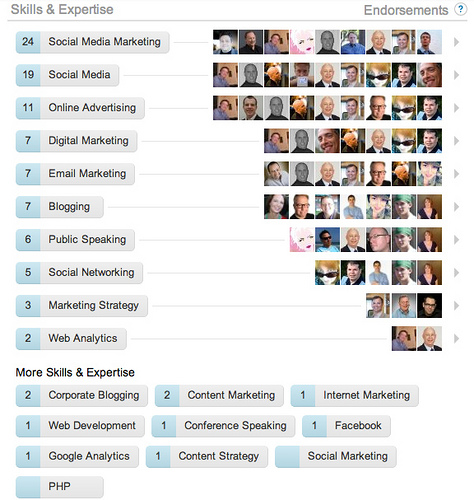
\includegraphics[width = 0.6\columnwidth]{linkedin-endorsements.jpg}
\centering
\caption{The Endorsement System in LinkedIn. A list of User Profile Pictures on the Right of Each ``Skills \& Expertise'', and Number on the Left Indicates How Many Connections in Their Social Network Have Certified This Item of Skill \cite{endorsement}.}
\label{endorsement}
\end{figure}

However, this type of evaluation of expertise can be very easily manipulated,  such as Twitter where users can purchase followers by number. In a previous study \cite{marlow2013activity}, user study participants have already mentioned that popularity is an indicator but not always enough to evaluate the quality of work. We argue the \textit{endorsement} on LinkedIn is also an indicator of popularity but on the skills and expertise of a developer.

In the future study, we purpose to carefully integrate the user rating and popularity based expertise evaluation with the automated techniques which mostly retrieve the activity history of a developer. However, we need to find a balance between employing user feedback and the historical data, but avoid over-reliance on either single data source.

\section{Paradox of Expertise}

The ultimate goal of locating expert is to find someone who is qualified to perform a job or task. It is non-trivial to determine the high-level goal of locating expertise firstly. However, even if experts have experienced so much in the past, when it comes to a specific task that requires to share expertise, such as training and coaching new employers, the person with highest expertise may not be the best candidate for performing these tasks due to the paradox of expertise \cite{dror2011paradox}, since their own experience and capacity \cite{liu2013expertise} bias them.

Experts think differently from novices. Their above-average performances in information processing often result from a pre-determined and routine mechanism. This mechanism is highly effective but also restricts the flexibility and control while expressing and articulating their specialties \cite{dror2011paradox}. For example, one of the best basketball players in the history, Michael Jordan, has never been a head coach of any basketball teams which, in fact, is determined by his incredibly high motion expertise in basketball, and it restricts his expression for his drills in playing basketball game e.g., Michael may believe dunking basketball over his opponent is an easy task, which is biased opinion due to his superior athleticism \cite{staff_nba.com_2017}. \textcolor{red}{this example does not fit your argument, it merely says gifted persons cannot transfer their  talent to ordinary people, but has nothing with the ``mechanism''}

In the study of Dror et al. \cite{dror2011paradox}, they claim one of the major reasons causing this paradox is the substantial amount of training that expert has received. Once forming an automated routine, their expertise is not easily accessible, and spending effort for accessing this effort degrades experts' performance \cite{flegal2008overthinking}. Therefore, expertise location studies need to consider this ``paradox'' of expert, and while locating expertise for expertise sharing tasks, novices may help experts to avoid this paradox. For example, \textit{Arthur Andersen LLP}\footnote{Arthur Andersen LLP was one of the largest accounting firms in the US} allocates their new hires called ``green beans'', into expert teams \cite{greenbeans}. These ``green beans'' ask basic questions such as the definition of terminologies, which helps the experts access their expertise when green beans ask questions \cite{kelly2009leadership}.

\section{Guiding Entry-level Novices}

Conventional expertise location techniques are usually employed in recommending people for performing specific software engineering task, and also in hiring, training and allocating software talents \cite{bergersen2014construction}. However, as open source software is playing an essential role in the software industry,  and due to its voluntary attribute \cite{shah2006motivation}, it is non-trivial to guide and encourage more participants to the community. However, newcomers of open source projects are facing various barriers to entering the community.

Past research by \citeauthor{STEINMACHER201567} has identified five main categories of these barriers \cite{STEINMACHER201567}. The major categories of these barriers are:

\begin{itemize}
    \item \textit{Technical Hurdles}: difficulties in understanding the code or setting up the workspace and environment.
    \item \textit{Documentation}: difficulties in understanding the project.
    \item \textit{Social interactions}: communication issues with the previous contributors of the project.
    \item \textit{Newcomers previous knowledge and expertise}: similar to technical hurdles, but more focusing on the newcomer's technical expertise such as experience in software engineering practice.
    \item \textit{Starting point}: difficulties in finding a mentor or entry-level task to start.
\end{itemize}

Except for the difficulty in social interaction, other barriers can be addressed or alleviated by sophisticated expertise location systems, particular finding a mentor with the required expertise to guide or help the novice to perform the technical task \cite{begel2008novice}. Further, to support newcomers to find the available expertise in the project and then enter the community for contribution, it also shows the non-trivial requirement of the expertise location systems which is including the constraints of the others such as their availability.

% do not use awareness information for constraints

% "disconnect" gap between doing it and what have done
\section{Limitations}

In this study, we reviewed the expertise location approaches and systems in Software Engineering and Computer Supported Collaborative Work based on our research questions. However, during our research procedure, we found early cognitive studies are not only focused on and limited to the field of Software Engineering. Though there are early studies about the relation between the information processing ability and programming expertise in the software engineering practice, we are not able to locate any studies that aimed to systematically build theories for measuring the expertise level for software engineering personnel. Due to the scope of this study, we only focus the papers in the field of Software Engineering and Computer Supported Collaborative Work; we may miss the progress in cognitive studies which analyze expert behaviors and characteristics. In the future study, we also intend to explore studies from other research subjects other than these two we have already reviewed in this study, particularly for field in management, organizational and cognitive science. Besides, we find related literature is not limited to the form of paper publications. There are lots of valuable resources in books \cite{ericsson2006cambridge, Simon:1996:SA:237774}, and we intend to include these resources as well.
\chapter{Conclusion}

In this study, we reviewed 48 primary studies about expertise location approaches and systems in the field of Software Engineering and Computer Supported Collaborative Work. We found that the conclusions in software engineering are similar to early cognitive research on expert performance. Moreover, we found several categories of expertise location approaches and systems measuring the expertise level based on the previous experience of developers which results in a disconnect between early cognitive expertise research and automated location techniques in Software Engineering practice. Further, we found the granularity of model for measuring expertise in these location techniques tend to be more focused on micro low-level tasks over the years, and it is challenging to evaluate the measurement of expertise and location approach in the real-world context. Finally, we conclude our findings and provide a series of discussions on future directions for expertise location studies in Software Engineering.
% ... and so on

% These commands fix an odd problem in which the bibliography line
% of the Table of Contents shows the wrong page number.
\clearpage
\phantomsection

% "References should be formatted in style most common in discipline",
% abbrv is only a suggestion.
% \bibliographystyle{plainnat}
\bibliographystyle{IEEEtranSN}
\bibliography{thesis}

% The Thesis Manual says not to include appendix figures and tables in
% the List of Figures and Tables, respectively, so these commands from
% the caption package turn it off from this point onwards. If needed,
% it can be re-enabled later (using list=yes argument).
\captionsetup[figure]{list=no}
\captionsetup[table]{list=no}

% If you have an appendix, it should come after the references.
% % The original template (from Trevor) had a custom \appendix command,
% but I found it to break figure/table counters. I'm not sure how
% reliable my fix is, so I ended up reverting back to the standard
% latex version, and renaming the custom command to \myappendix.  You
% can try both and see how things work out:
% 1) Call \appendix once, and then make each appendix a \chapter
% 2) Call \myappendix once, and then make each appendix a \section.

\appendix
\chapter{Appendix Title}

Supplementary material goes here. See for instance Figure
\ref{fig:quote}.

\section{Lorem Ipsum}

dolor sit amet, consectetur adipisicing elit, sed do eiusmod tempor
incididunt ut labore et dolore magna aliqua. Ut enim ad minim veniam,
quis nostrud exercitation ullamco laboris nisi ut aliquip ex ea
commodo consequat. Duis aute irure dolor in reprehenderit in voluptate
velit esse cillum dolore eu fugiat nulla pariatur. Excepteur sint
occaecat cupidatat non proident, sunt in culpa qui officia deserunt
mollit anim id est laborum.

\begin{figure}
  \centering
  \begin{tabular}{l}
    ``I am glad I was up so late,\\
    \quad{}for that's the reason I was up so early.''\\
    \em \footnotesize William Shakespeare (1564-1616), British
    dramatist, poet.\\
    \em \footnotesize Cloten, in Cymbeline, act 2, sc. 3, l. 33-4.
  \end{tabular}
  \caption{A deep quote.}
  \label{fig:quote}
\end{figure}


%%% Local Variables: ***
%%% mode: latex ***
%%% TeX-master: "thesis.tex" ***
%%% End: ***


\end{document}
